\documentclass[10pt, conference, letterpaper]{IEEEtran}

\usepackage{epstopdf}%
\usepackage{algorithm}
\usepackage{algorithmic}
\usepackage{amsfonts}
\usepackage{stmaryrd}
\usepackage{cite}
\usepackage{color}
\usepackage{multirow}
\usepackage{graphicx,times,amsmath} % Add all your packages here
\usepackage[center,normal]{caption}
\usepackage{amssymb}
\usepackage{amsthm}
\newtheorem{proposition}{Proposition}
\newtheorem{corollary}{Corollary}
\newtheorem{observation}{Observation}
\newtheorem{result}{Result}
\newtheorem{theorem}{Theorem}
\newtheorem{lemma}{Lemma}
\newtheorem{definition}{Definition}
\usepackage{enumitem}
\usepackage{datetime}
\usepackage{url}
\settimeformat{hhmmsstime}
\renewcommand{\algorithmicrequire}{ \textbf{Input:}} %Use Input in the format of Algorithm
\renewcommand{\algorithmicensure}{ \textbf{Output:}} %Use Output in the format of Algorithm


\begin{document}

\title{Clockwork: Scheduling Cloud Requests \\in Mobile Applications}

\author{\IEEEauthorblockN{Yanjiao Chen$^{\ddagger}$, Zixuan Yu$^\S$, Baochun Li$^\S$} \\
	\IEEEauthorblockA{$^\S$State Key Lab of Software Engineering, School of Computer, Wuhan University, China\\
		$\S$Department of Electrical and Computer Engineering, University of Toronto\\		
		Email: $\ddagger$chenyanjiao@whu.edu.cn, $\S$\{zixuan.yu, bli\}@ece.toronto.edu}
}

\maketitle
\begin{abstract}
It is essential for mobile application developers to manage backend resources to serve dynamic user requests from the frontend. For a typical mobile application, the rate at which the user requests arrive at the backend fluctuates dramatically.  However, it is difficult or expensive to frequently adjust the capacity of the backend to meet the request demand.  In this paper, we present \emph{Clockwork}, a third-party cloud service, which smooths the demand profile by redistributing delay-tolerant requests and prioritizing delay-sensitive requests, so that sufficient capacity can be provided with reduced cost and wastage. To begin with, Clockwork plans the optimal backend capacity on a relatively long timescale based on future demand estimated by machine learning algorithms. We discuss pros and cons of various simple machine learning algorithms and advanced deep learning algorithms, in terms of their prediction accuracy and training time. Then, Clockwork schedules user requests on a shorter timescale through a fair and Pareto-optimal rate allocation.  We implemented a fully-functional prototype of Clockwork on cloud servers and user mobile devices. The experimental results show that Clockwork can effectively help developers cut cost, as well as improve the backend utilization.          
\end{abstract}
\section{Introduction}

The market for mobile applications is booming. In 2015, global application downloads are estimated to be $179$ billion \cite{downloads}, generating $\$45$ billion revenues \cite{revenue} and involving $5.5$ million developers \cite{developer}. To compete for market share and profits, application developers are motivated to provide quality service with reduced cost.

Backend provisioning is one of the fundamental concerns for developers, as all user requests from the frontend of an application need to be handled by the backend. Developers can either use Mobile-backend-as-a-Service (MBaaS) or build their own backends on cloud platforms (such as Amazon EC2). In the former case, developers can directly enjoy backend services offered by MBaaS providers, who charge fees based on the number of requests sent to the MBaaS backend.  In the latter case, developers can construct their backends using instances, and pay for their usage.

One of the biggest challenges facing backend provisioning is a mismatch between timescales of request demand variance and backend resource availability. The rate at which user requests arrive at the backend varies from second to second, but developers can neither change the MBaaS service plan nor adjust instance configurations at such a fine granularity of time. Though Amazon EC2 also provides auto-scaling mechanisms, it requires developers to determine how many instances to add or reduce, and it takes time to boot up or shut down computers. Rather than trying to let the backend capacity closely \emph{track} the demand profile, which is difficult or even impossible to realize, we explore a new way of backend provisioning. We \emph{smooth} the demand profile by redistributing delay-tolerant requests and prioritizing delay-sensitive requests, which potentially lightens the burdens on the backend and saves money for developers.

\begin{figure}[t]
	\centering
	\hspace{-0.4cm}
	\begin{minipage}[t]{1.7in}
		\centering
		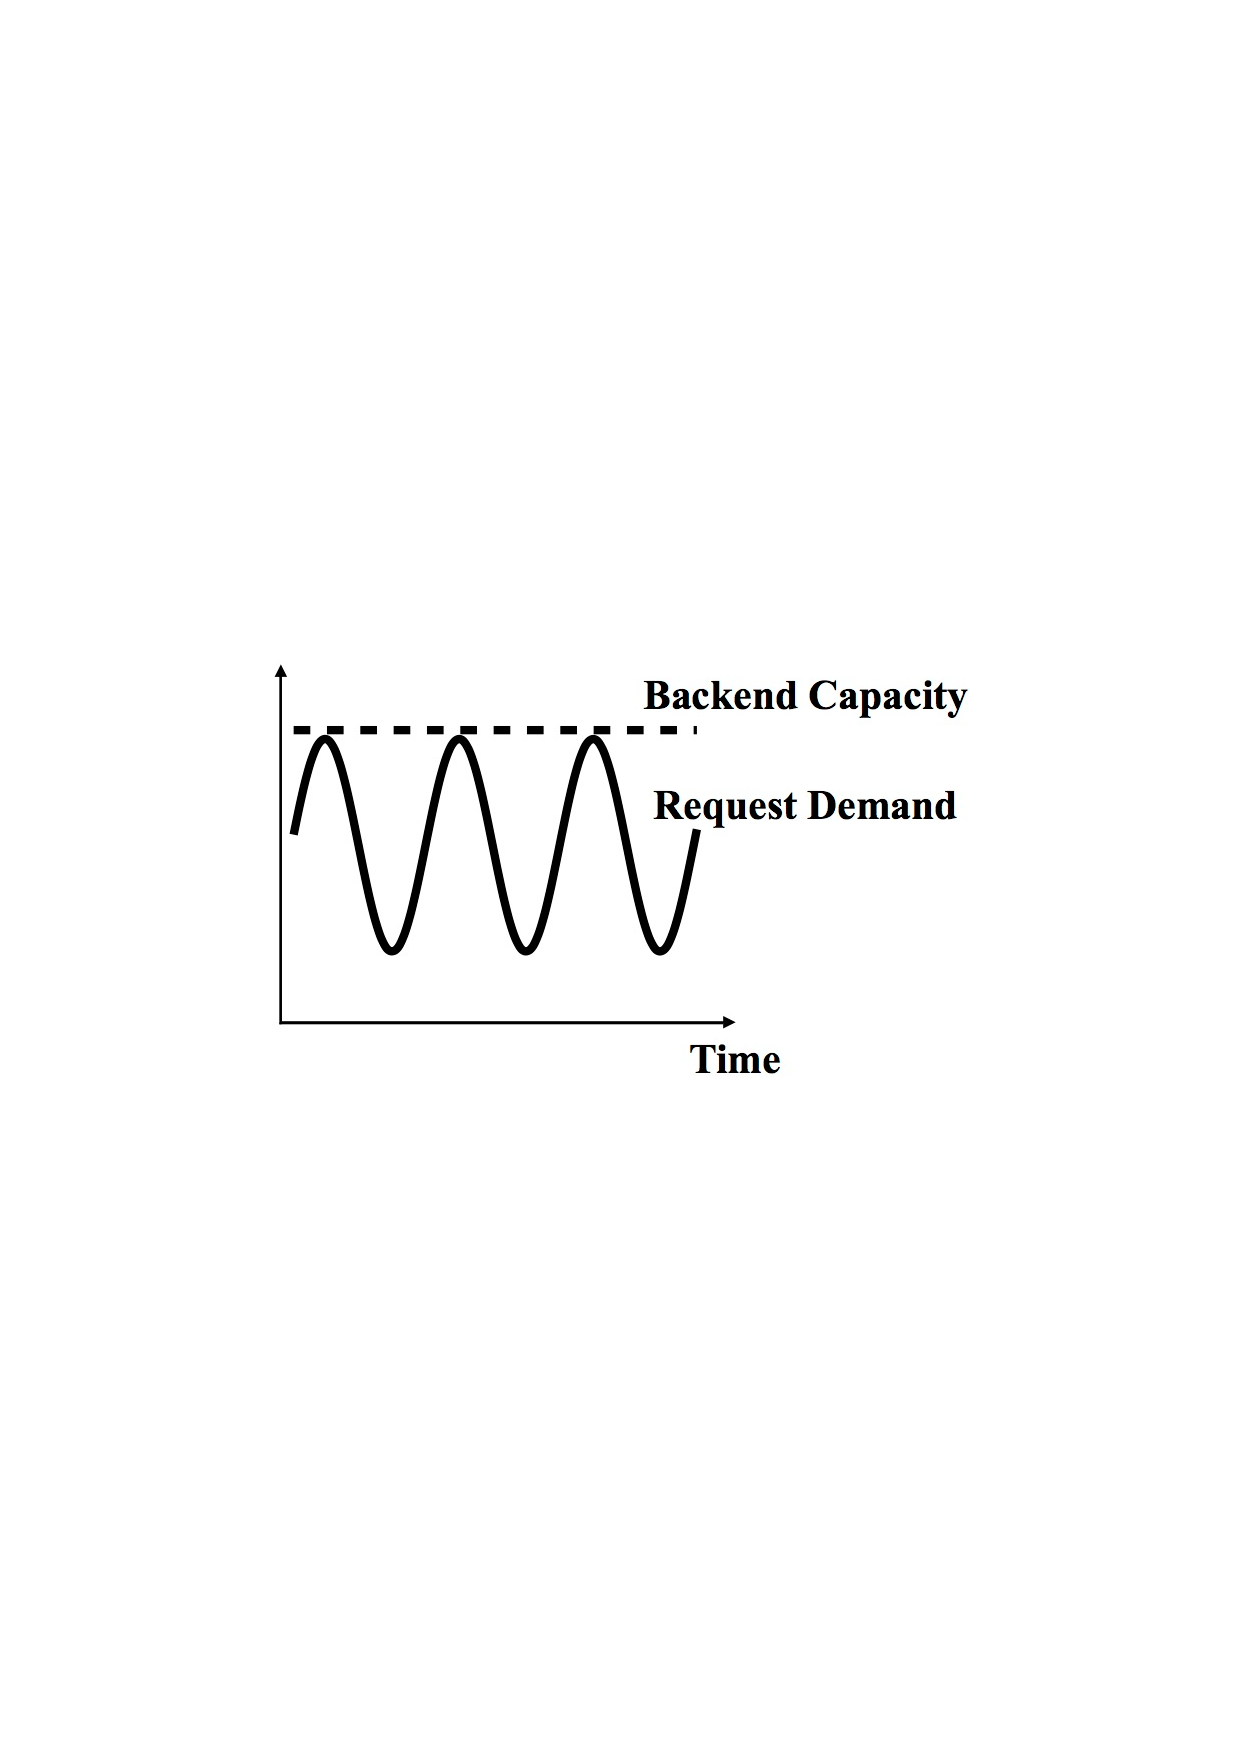
\includegraphics[trim=45mm 110mm 45mm 110mm, clip,width=1.7in]{figs/intro1}\\
		\centerline{(a) Provisioning for}
		\centerline{peak demand}
	\end{minipage}
	\hspace{-0.1cm}
	\begin{minipage}[t]{1.8in}
		\centering
		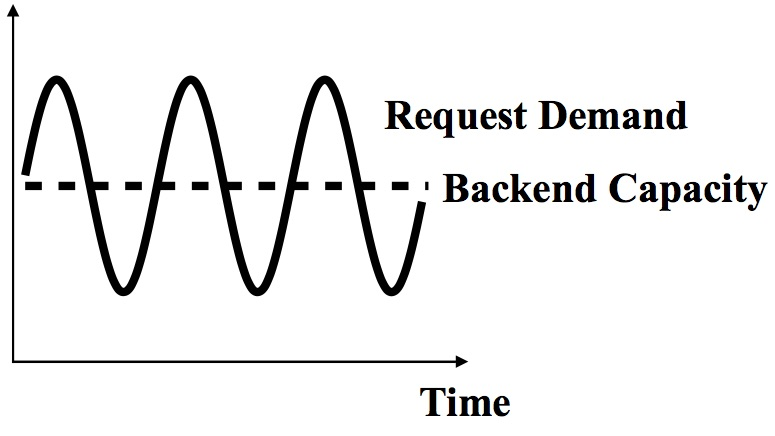
\includegraphics[trim=40mm 110mm 40mm 110mm, clip,width=1.8in]{figs/intro2}\\
		\centerline{(b) Provisioning for}
		\centerline{average demand}
	\end{minipage}
	\hspace{-0.cm}
	\begin{minipage}[t]{1.8in}
		\centering
	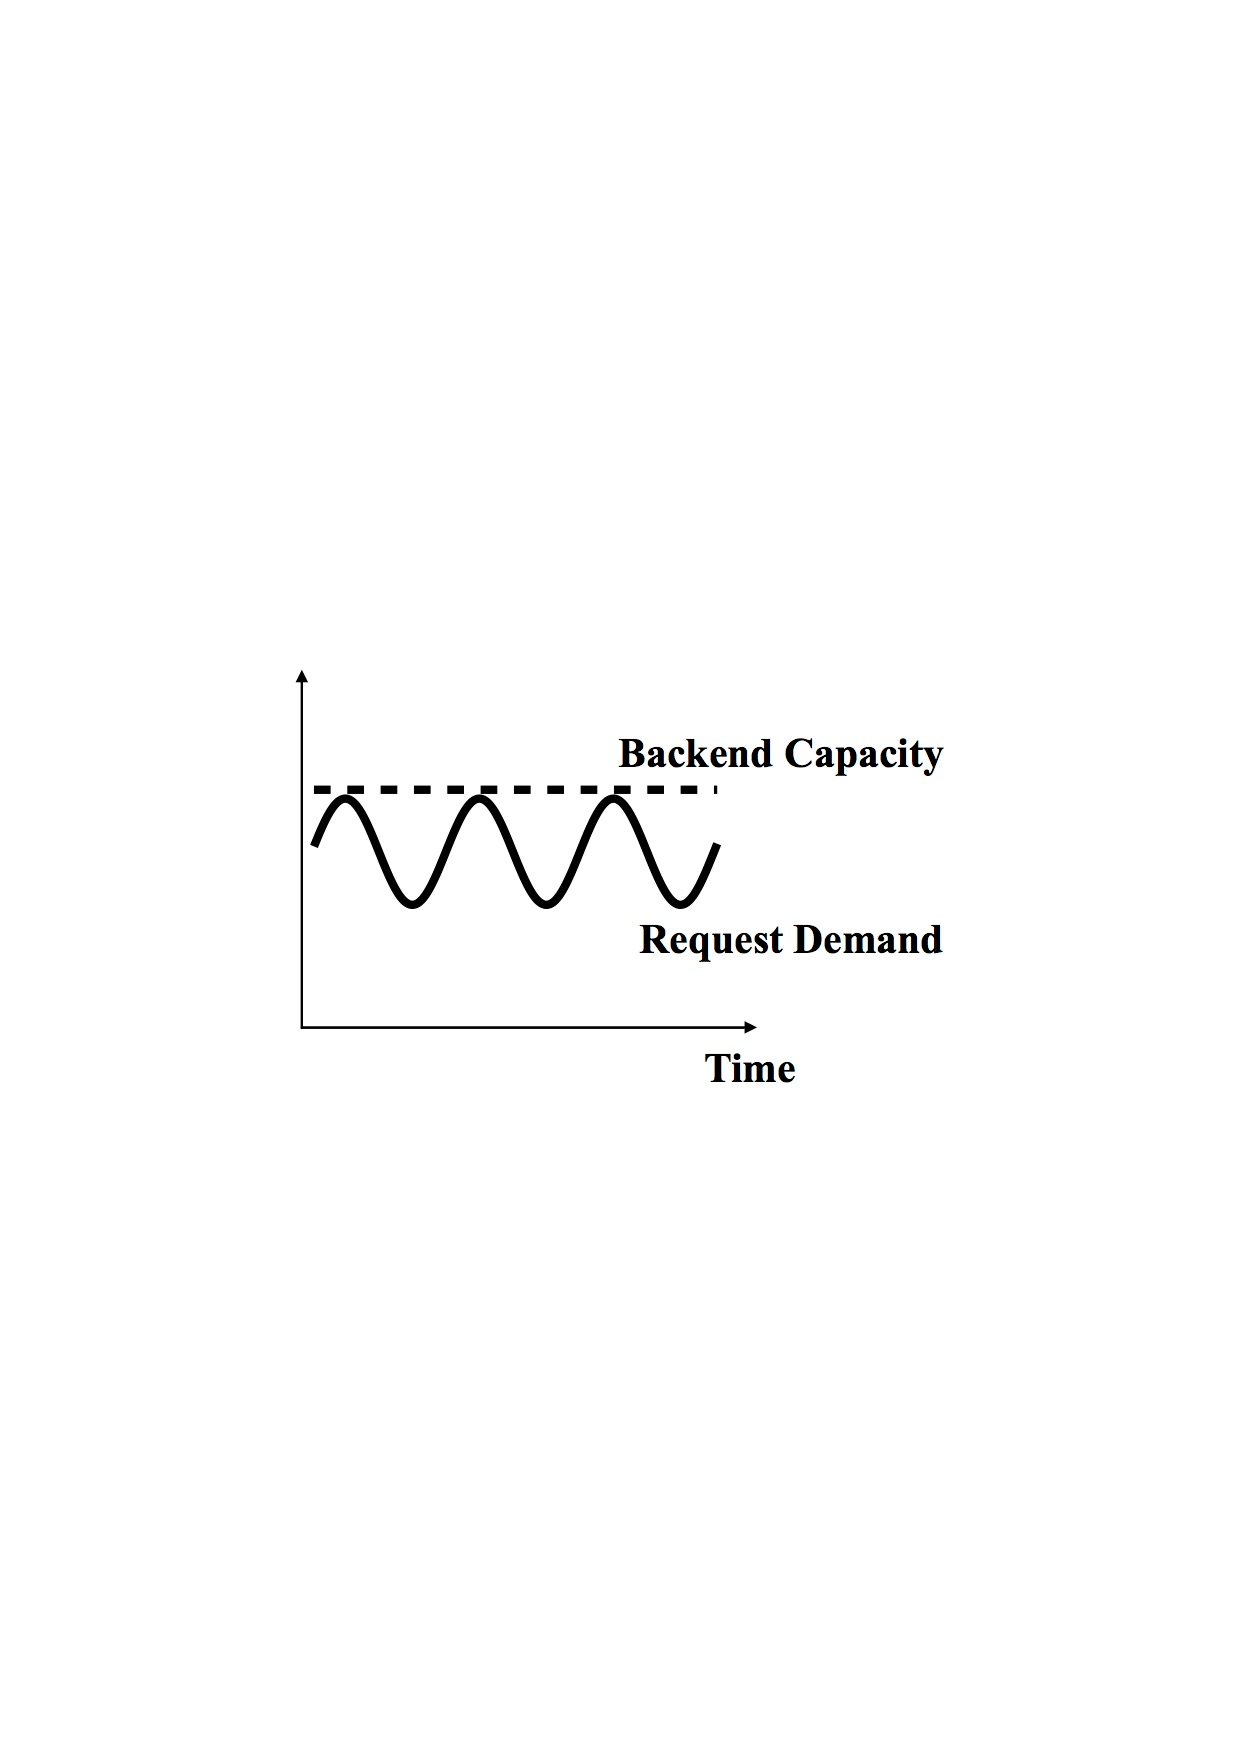
\includegraphics[trim=50mm 110mm 45mm 110mm, clip,width=1.8in]{figs/intro3}\\
		\centerline{(c) Clockwork}
	\end{minipage}
	\caption{Backend provisioning comparison.} \label{fig:intro}
\end{figure}

To achieve such a goal, we present Clockwork, a third-party cloud service designed to help developers manage backend provisioning. Clockwork features a two-tier architecture: backend capacity planning on a long timescale, and rate-based request scheduling on a short timescale. Both tiers are indispensable in helping developers maintain a sufficient and cost-effective backend. As shown in Fig.~\ref{fig:intro}(a), if the backend capacity caters to the peak demand to avoid any performance degradation, there will be a considerable wastage of resources and money. Nevertheless, if the backend capacity falls short of the peak demand, as shown in Fig.~\ref{fig:intro}(b), some requests will have to be dropped or experience unacceptably long processing times. In comparison, Clockwork schedules requests according  to delay tolerance, as shown in Fig.~\ref{fig:intro}(c), thus flattening the request demand and slashing the required backend capacity.


There are several challenges facing the implementation of Clockwork. To plan for the long-term backend capacity, it is crucial to have an accurate prediction of the future request demand. There is a wide variety of machine learning algorithms for data prediction, each of which has their advantages and disadvantages. We compare the prediction accuracy and training time of four machine learning algorithms (Section \ref{sec:predict}). It is shown that deep learning algorithms, including convolutional neural networks and deep belief networks, yield better prediction results but require a much longer time to train than simpler machine learning algorithms, such as logistic regression and multilayer perceptron. With the estimated future demand, the Clockwork derives the optimal backend capacity that minimizes developer's cost, while conforming to the constraint on request delay  (Section \ref{sec:plan}).

Given the long-term capacity, to ensure that the backend is not overwhelmed by instant request demand, we adopt a rate-based resource allocation strategy (Section \ref{sec:rateall}). Clockwork centrally assigns rates to users based on the quantity and delay tolerance of their requests, then individual users autonomously schedule their own requests. We build a network utility maximization (NUM) model to decide the rate allocation, which is proved to be fair and Pareto-optimal.



We have implemented the server-side of Clockwork using the Amazon Web Service (AWS), and the client-side of Clockwork on iOS-based mobile devices. We present the implementation details (Section \ref{sec:implementation}) and evaluate the performance of Clockwork by a small-scale pilot experiment and a large-scale simulation (Section \ref{sec:experiment}). The results show that Clockwork can help developers substantially cut down the backend cost, as well as improve the backend utilization.













\begin{figure}[t]
	\center
	\hspace{-0cm}
	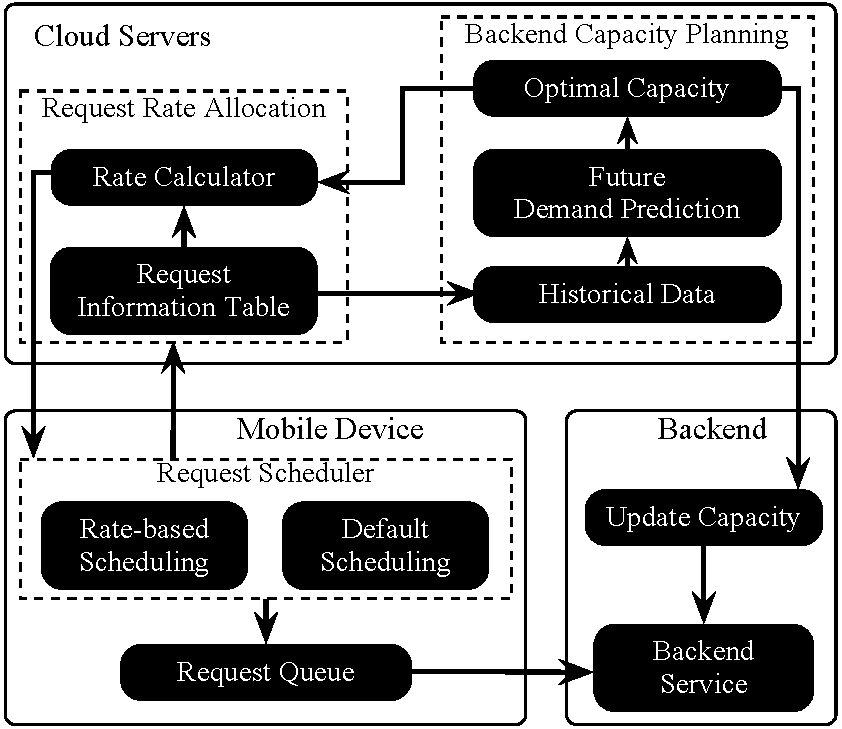
\includegraphics[width=3.3in]{figs/sys}
	\caption{Architecture of Clockwork.} \label{fig:sys}
	\vspace{-0.cm}
\end{figure} 
\section{Clockwork: Motivations and Architecture}\label{sec:background}

\begin{figure}[t]
	\centering
	\hspace{-0.5cm}
	\begin{minipage}[t]{1.7in}
		\centering
		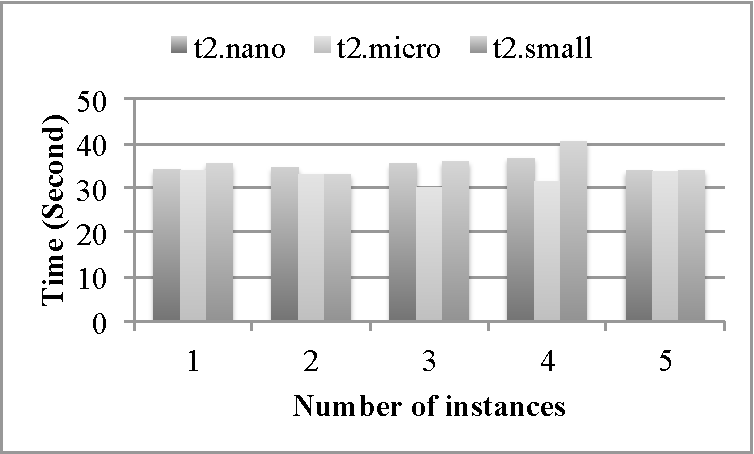
\includegraphics[trim=5mm 5mm 5mm 5mm, clip,width=1.7in]{figs/end}\\
		\centerline{\small{(a) Launch instances}}
	\end{minipage}
	\hspace{-0.2cm}
	\begin{minipage}[t]{1.7in}
		\centering
		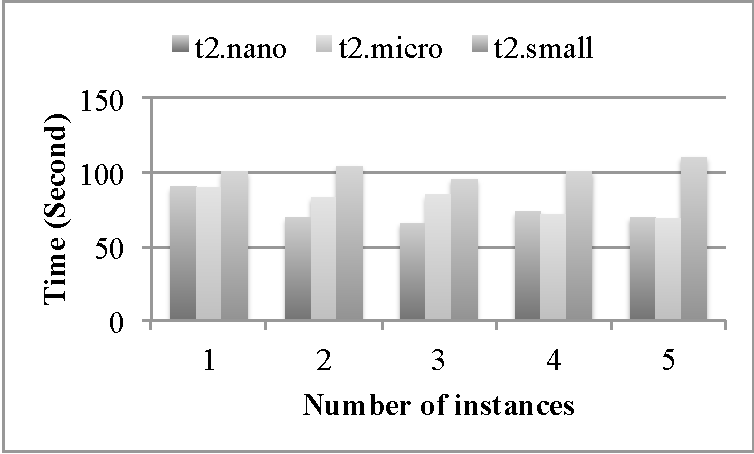
\includegraphics[trim=5mm 5mm 5mm 5mm, clip,width=1.7in]{figs/start}\\
		\centerline{\small{(b) Terminate instances}}
	\end{minipage}
	\caption{Time for launching or terminate instances} \label{fig:instance}
\end{figure}

\begin{figure}[t]
	\center
	\hspace{-0cm}
	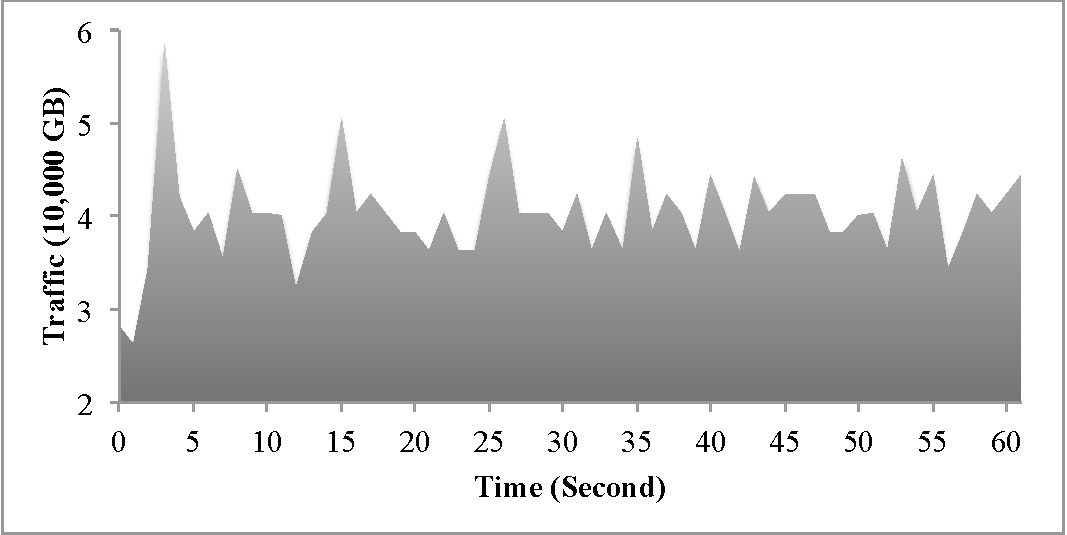
\includegraphics[trim=5mm 5mm 5mm 3mm, clip,width=3.3in]{figs/traffic}
	\caption{Network traffic fluctuations.} \label{fig:traffic}
	\vspace{-0.cm}
\end{figure} 

Mobile application development comprises two major parts: frontend design and backend support. Simply put, the frontend of an application is what users can see and experience on their mobile devices. The frontend differentiates one application from another, thus it is vastly diversified for different applications. The backend of an application supports its frontend functionalities. When a user interacts with the application through the frontend, the corresponding operations are accommodated via API requests to the backend. Typical API requests of a mobile application include queries, saves, and logins, amongst other kinds of operations invoked by users to perform a task. Some requests are urgent, while some others are delay-tolerant. Take social messaging applications as an instance. The request of \emph{sending a message} is urgent and should be served straightaway, while the request of \emph{updating the user profile} can wait to be served later. 

In this paper, we focus on the backend of the application development, whose cost model is more common across all applications. Mobile application developers can use the ready-made and customizable backend provided by MBaaS or build their own backends on cloud platforms such as Amazon EC2. 

MBaaS providers, such as Appcelerator, appery.io, and Kumulos, charge developers based on the number of API requests sent by users to the MBaaS backend. More specifically, the developer should subscribe to a service plan, usually on an hourly or monthly basis. The service plan specifies the limit on the maximum number of requests that can be sent within a unit time, e.g., one minute. If such a limit is hit, extra requests will be discarded with error messages to users. A service plan with a higher request limit will cost more. 

If a developer utilizes Amazon EC2 to set up the backend, her cost depends on the number and the type of instances that are launched. For example, a t2.nano instance with 1 CPU and 0.5GB memory costs $\$0.0059$ per hour, and a t2.small instance with 1 CPUs and 2GB memory costs $\$0.023$ per hour.  The payment is prorated by the hour. This indicates that once a developer turns on a t2.large instance, she will immediately be charged $\$0.094$, even if she doesn't plan to use the instance for the entire hour. 

Fig.~\ref{fig:traffic} illustrates the world network traffic by the second\footnote{http://www.internetlivestats.com/}, from which we can infer that there is a dramatic fluctuation in mobile backend traffic. The demand peak may be much higher than the average, but is only momentary. In contrast, developers can only change MBaaS service plan on an hourly basis. As for cloud services, Fig.~\ref{fig:instance} shows that it takes around one minute to launch or terminate an instance, and a new instance is charged for a full hour even if it is only needed for a short period of time. 



To address the above challenge, the architecture of Clockwork consists of two major modules: backend capacity planning and request rate allocation, as shown in Fig.~\ref{fig:sys}. Backend capacity planning is conducted on a relatively long timescale, e.g., per hour, since it is either difficult or costly to frequently change the backend capacity. Request rate allocation is performed on a short timescale, e.g., per minute, based on the dynamics of request demand. 

   


 






\section{Backend Capacity Planning} \label{sec:theory}




     

\subsection{Backend Capacity Optimization}\label{sec:plan}

Without loss of generality, we define the backend capacity as the maximum number of requests that can be served per minute, which is directly linked to the cost of the backend (e.g., to pay for the MBaaS service plan or the instances on Amazon EC2). We assume that the developer is able to adjust the backend capacity on an hourly basis. Let $N$ denote the required backend capacity, to be determined by the optimization model. The developer classifies all possible requests of the application into $K$ types, according to their delay tolerance. For example, there can be $K=3$ types of requests: urgent, medium, and delay-tolerant. An hour consists of $i = 1,2,...,60$ minutes, during which the backend capacity is fixed. Let $n_i^k$ denote the estimated number of type $k$ requests that will arrive at the $i$-th minute in the next hour. In this section, we assume that  $n_i^k, i\in[1,60], k \in[1,K]$ are available as inputs to the optimization model, and we will discuss how to predict $n_i^k$ in details in the next section. Without Clockwork, to guarantee the performance of the backend, the developer has to make sure that the backend capacity is greater than the peak demand, i.e., $N \ge \max_i\sum_k n_i^k$. We will show that such over-provisioning is unnecessary with the request scheduling mechanism of Clockwork.  


We make the simplified assumption that all requests generated in a specific hour will be served within that hour. In other words, during the current hour, the backend will neither serve requests from the previous hour, nor put off requests to the next hour. At the $i$-th minute, let $\delta_{ij}^k \in [0,1]$ denote the proportion of the $n_i^k$ requests that will be postponed to the $j$-th minute. We have $i \le j \le 60$, and $\delta_{ii}^k$ is the proportion of requests that are not delayed.  All requests to be served at the $j$-th minute, denoted by $N_j$, include those deferred from the previous minutes to the $j$-th minute, and those generated and instantly served in the $j$-th minute, i.e., $N_j = \sum_{i=1}^{j-1}\sum_{k=1}^K\delta_{ij}^k n_i^k + \sum_{k=1}^K\delta_{jj}^k n_j^k = \sum_{i=1}^{j}\sum_{k=1}^K\delta_{ij}^k n_i^k$. To guarantee the performance of the backend, its capacity should be larger than the peak demand after request scheduling, i.e., $N \ge \max_{j\in[1,60]}N_j$. 

Delaying requests will affect the user experience, thus the developer needs to have a control over how many and how long a certain type of requests can be delayed. Clockwork allows the developer to set the upper-bound of $\delta_{ij}^k$ as $\overline{\delta_{ij}^k}$, which depends on the request  type $k$ and the length of delay $j-i$. For instance, in a social messaging application, if  \emph{sending a message} is regarded as the most urgent type of requests and should not be delayed, the developer can simply set $\forall j > i,\overline{\delta_{ij}^{\textrm{send a message}}} = 0$; if no request should be delayed for more than half an hour, the developer can simply stipulate that $\forall k,\overline{\delta_{ij}^{k}} = 0, \textrm{if } j - i > 30$.     

As the backend cost will monotonically increase with the backend capacity, we set the objective of Clockwork as to minimize the required backend capacity, without violating the constraint on $\delta_{ij}^k$ designated by the developer.

\begin{align}\label{equ:opt}
\min\limits_{\delta_{ij}^k}~ & N, \\
\textrm{subject to } & N \ge \max\limits_{j\in[1,60]}N_j, \label{equ:constraint0}\\
& N_j = \sum_{i=1}^{j}\sum_{k=1}^K\delta_{ij}^k n_i^k, \forall j,\label{equ:constraint1}\\
&\sum\limits_{j = i}^{60} \delta_{ij}^k = 1, \forall i, \forall k,\label{equ:constraint}\\
& 0\le \delta_{ij}^k \le \overline{\delta_{ij}^k}, \forall i, \forall j, \forall k.
\end{align}
Constraint (\ref{equ:constraint0}) guarantees that the backend capacity is large enough to meet the peak request demand. Constraint (\ref{equ:constraint1}) shows the number of requests per minute after scheduling. Constraint (\ref{equ:constraint}) ensures that all the requests initiated in the $i$-th minute are served, either instantly or in later minutes. The objective function is minimized through variables $\delta_{ij}^{k}$, and we can get the optimal backend capacity as $N^*  = \max_{j\in[0,60]}N_j^*$, in which $N_j^* = \sum_{i=1}^{j}\sum_{k=1}^K{\delta_{ij}^k}^* n_i^k$. The optimization problem (\ref{equ:opt}) is a linear programming problem, and can be solved by existing algorithms such as Simplex and Interior point algorithms. Fig.~\ref{fig:serviceplan2} gives an example of how the backend capacity planning of Clockwork works. It is shown that the demand profile is smoothed as Clockwork schedules requests to \emph{cut} the peak and \emph{fill} the valley.   



\begin{figure}[t]
	\center
	\hspace{-0.2cm}
	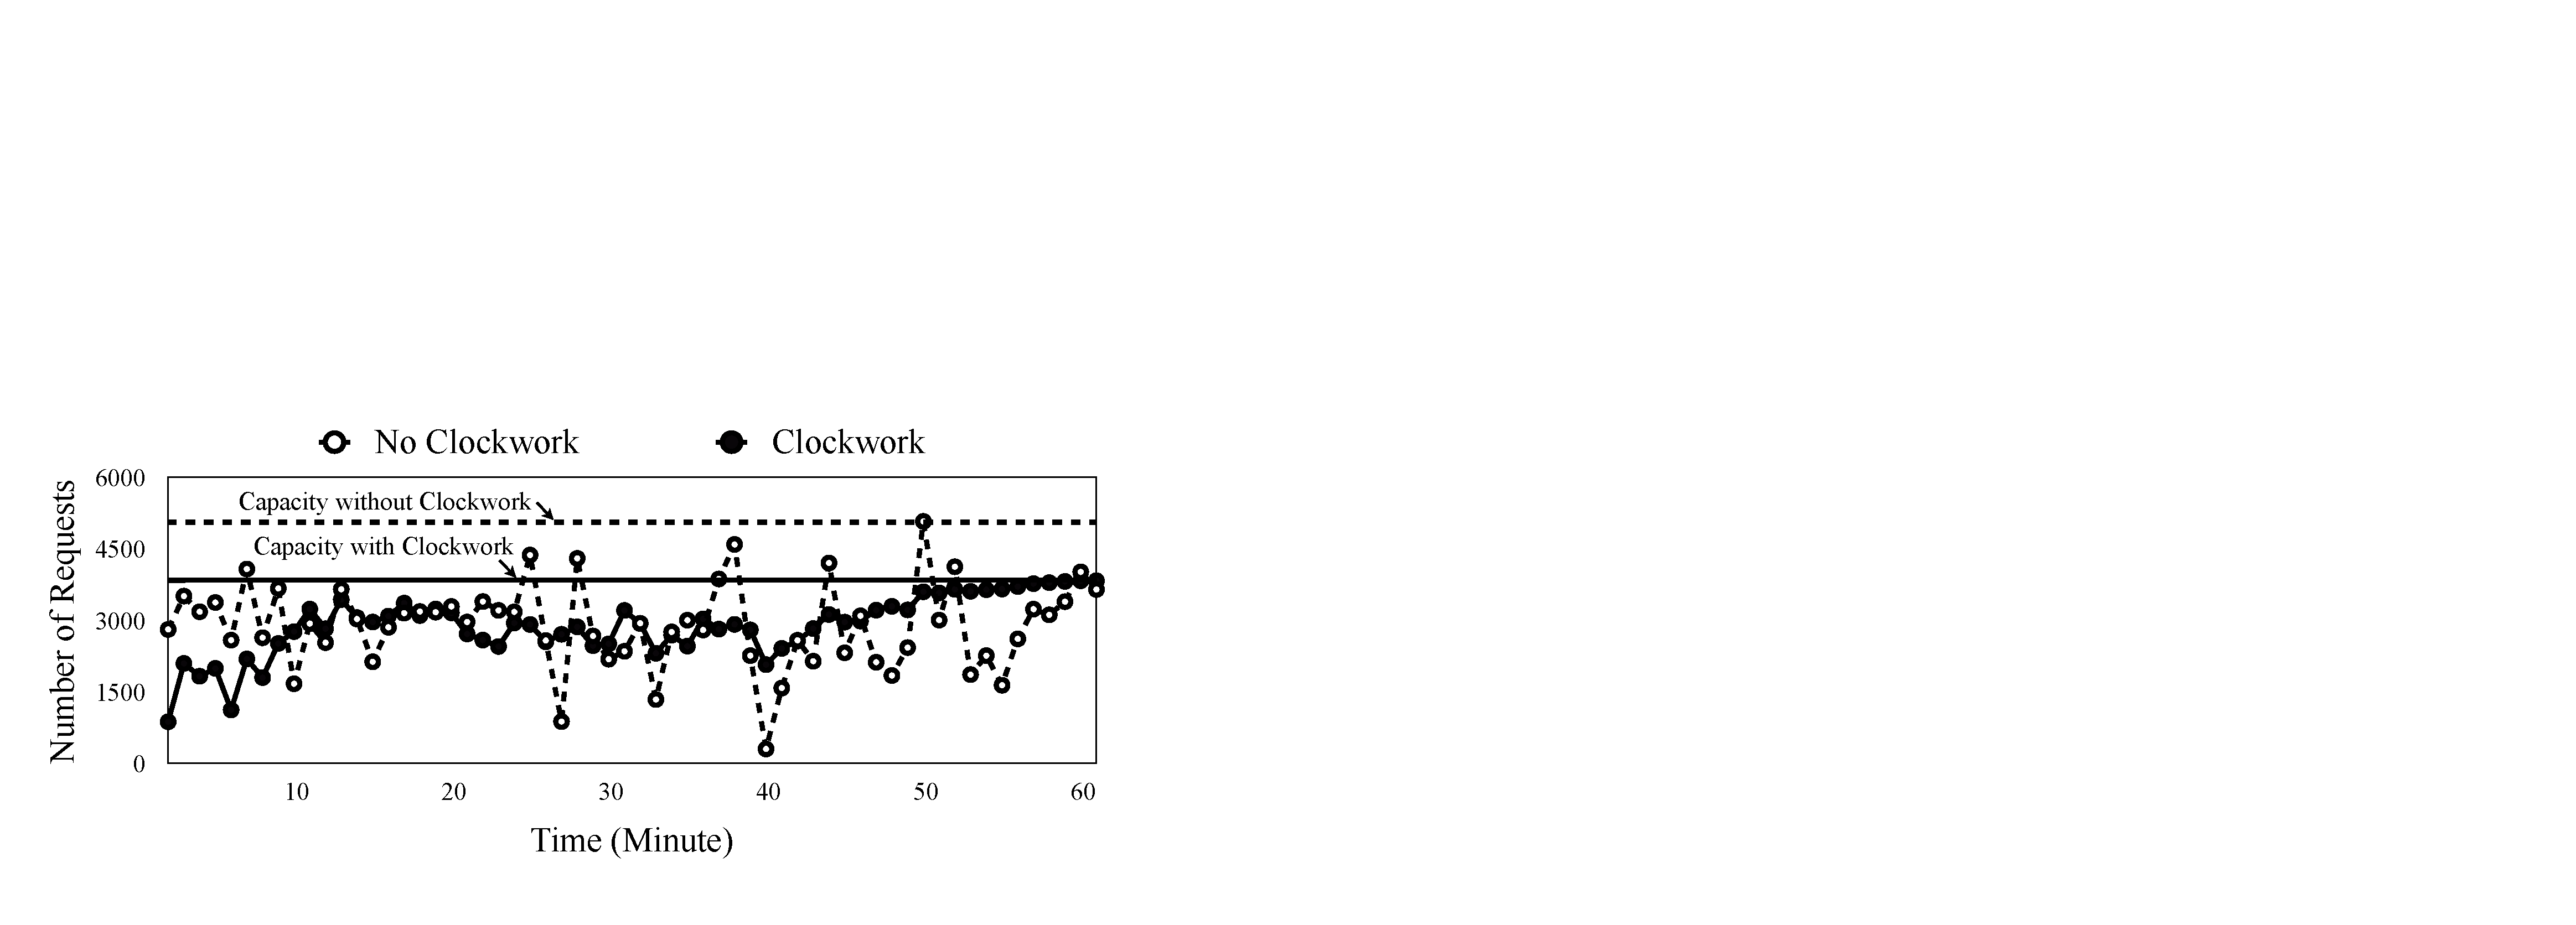
\includegraphics[trim = 0mm 0mm 0mm 0mm,clip,width=3.3in]{figs/cp1}
	\caption{Request demand smoothing by Clockwork.} \label{fig:serviceplan2}
\end{figure}	

\subsection{Future Demand Prediction}\label{sec:predict}

The optimization problem (\ref{equ:opt}) requires the input of $n_i^k$, the expected number of type $k$ requests generated at the $i$-th minute of the next hour, which can be learned from historical data using machine learning algorithms.  We focus on four widely-used  algorithms: logistic regression (LR), single-hidden-layer multilayer perceptron (sMLP), deep belief networks (DBN), and convolutional neural networks (CNN). Logistic regression and sMLP are simple machine learning models, while DBN and CNN are deep learning models. For simplicity, in this paper, we use these models for classification, while they can easily be adapted for regression. For instance, $n_i^k\in (1,100]$ and $n_i^k \in (100, 200]$ can be defined as class $1$ and class $2$, respectively. 

Historical data are collected in the form of the number of requests generated in each minute. The input vector $\pmb{x}$ to the machine learning model should contain the best predictors for $n_i^k$. Two potential factors need to be taken into consideration. One is \emph{temporal-proximity}, i.e., the most recent demand indicates the near future. The other is \emph{diurnal} effect, i.e., demands at the same time of each day have a similar trend. Therefore, we use the demand of the previous two hours and the demand at the same time of the previous two days as the input vector to predict $n^k_i$, i.e., $\pmb{x}=(n_{i-180}^k,\cdots, n_{i-61}^k, n_{i-1440-180}^k,\cdots,n_{i-1440+179}^k,\\ n_{i-1440*2-180}^k,\cdots n_{i-1440*2+179}^k)$, and $Y= n^k_i$. Furthermore, we normalize entries in the input vectors as $\pmb{x} \rightarrow \pmb{x}/\max\{n_i^k\}$, and discretize the output into $10$ levels for classification.  

We use synthetic datasets to evaluate the performance of the four machine learning models as follows. Assume that there are $100$ users, each generating requests according to a Poisson process. Without loss of generality, we only consider one type of requests. We first generate a series of values with a diurnal pattern (low demand at working time, and high demand at leisure time), to represent the request arrival rate at different time of a day for an average user. Then, we compute the arrival rate for each individual user by adding noise to the arrival rate of the average user. Aggregating the number of requests from all users at each minute yields the demand profile. We run the four machine learning algorithms on a MacBook Pro laptop with $2.9$ GHz Intel CPU and 8 GB memory.     


\begin{figure}[t]
	\center
	\hspace{-0.4cm}
	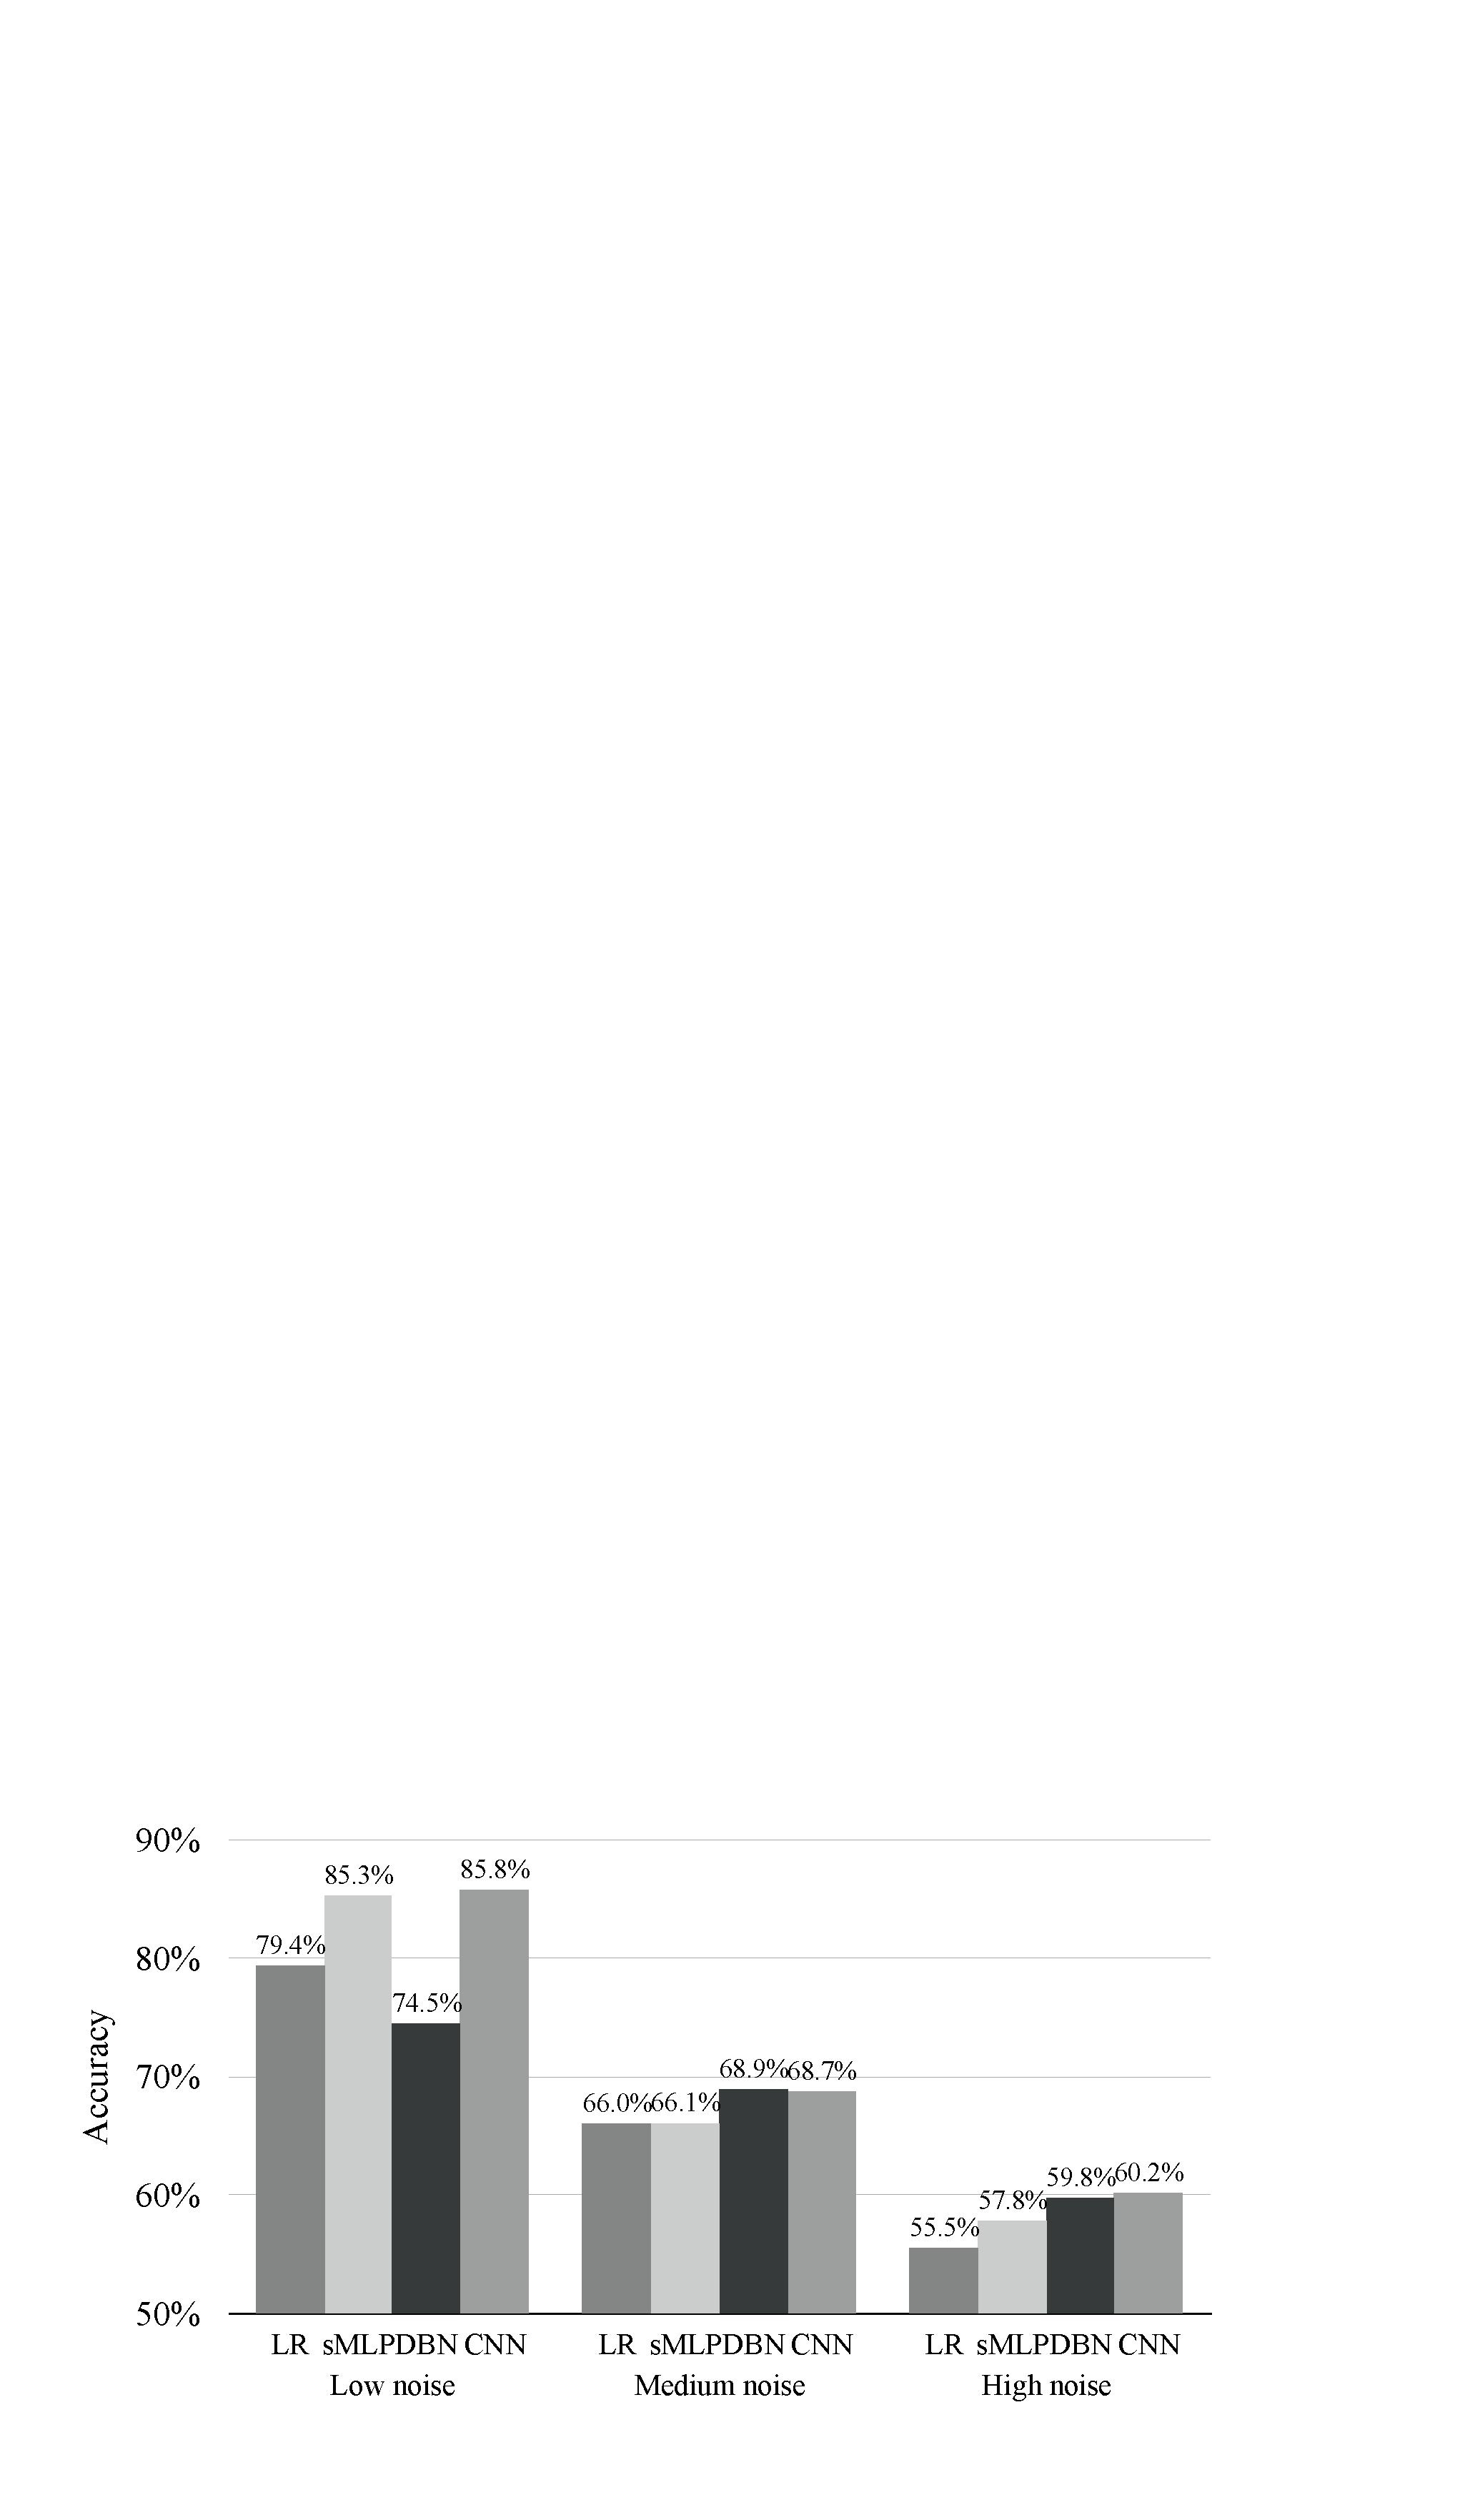
\includegraphics[trim = 0mm 0mm 0mm 12mm,clip,width=3.4in]{figs/acc}
	\caption{Prediction accuracy.} \label{fig:acc}
\end{figure}

As shown in Fig.~\ref{fig:acc}, deep learning models outperform simple models when the dataset is more noisy, since deep learning models are more powerful in discovering the intricate relationship between the input and the output. Unexpectedly, at the low noise level, DBN gives the worst prediction result, even inferior to the logistic regression model. One possible reason is that the complicated structure of DBN leads to the over-fitting problem. In other words, the model exaggerates the noise in the training data, instead of learning the general trend, therefore gives poor predictions when applied to the testing data. 

As shown in Fig.~\ref{fig:time}, the training time of deep learning models is far higher than that of simple models, which is not surprising since the deep learning models contain far more parameters to be learned. The training time of DBN and CNN also depends on the choice of the number of layers and neurons in each layer. Though the training time diverges considerably, given a new input, it takes almost the same time (less than a second) for the trained models of all four algorithms to yield the prediction result. 


\begin{figure}[t]
	\center
	\hspace{-0.4cm}
	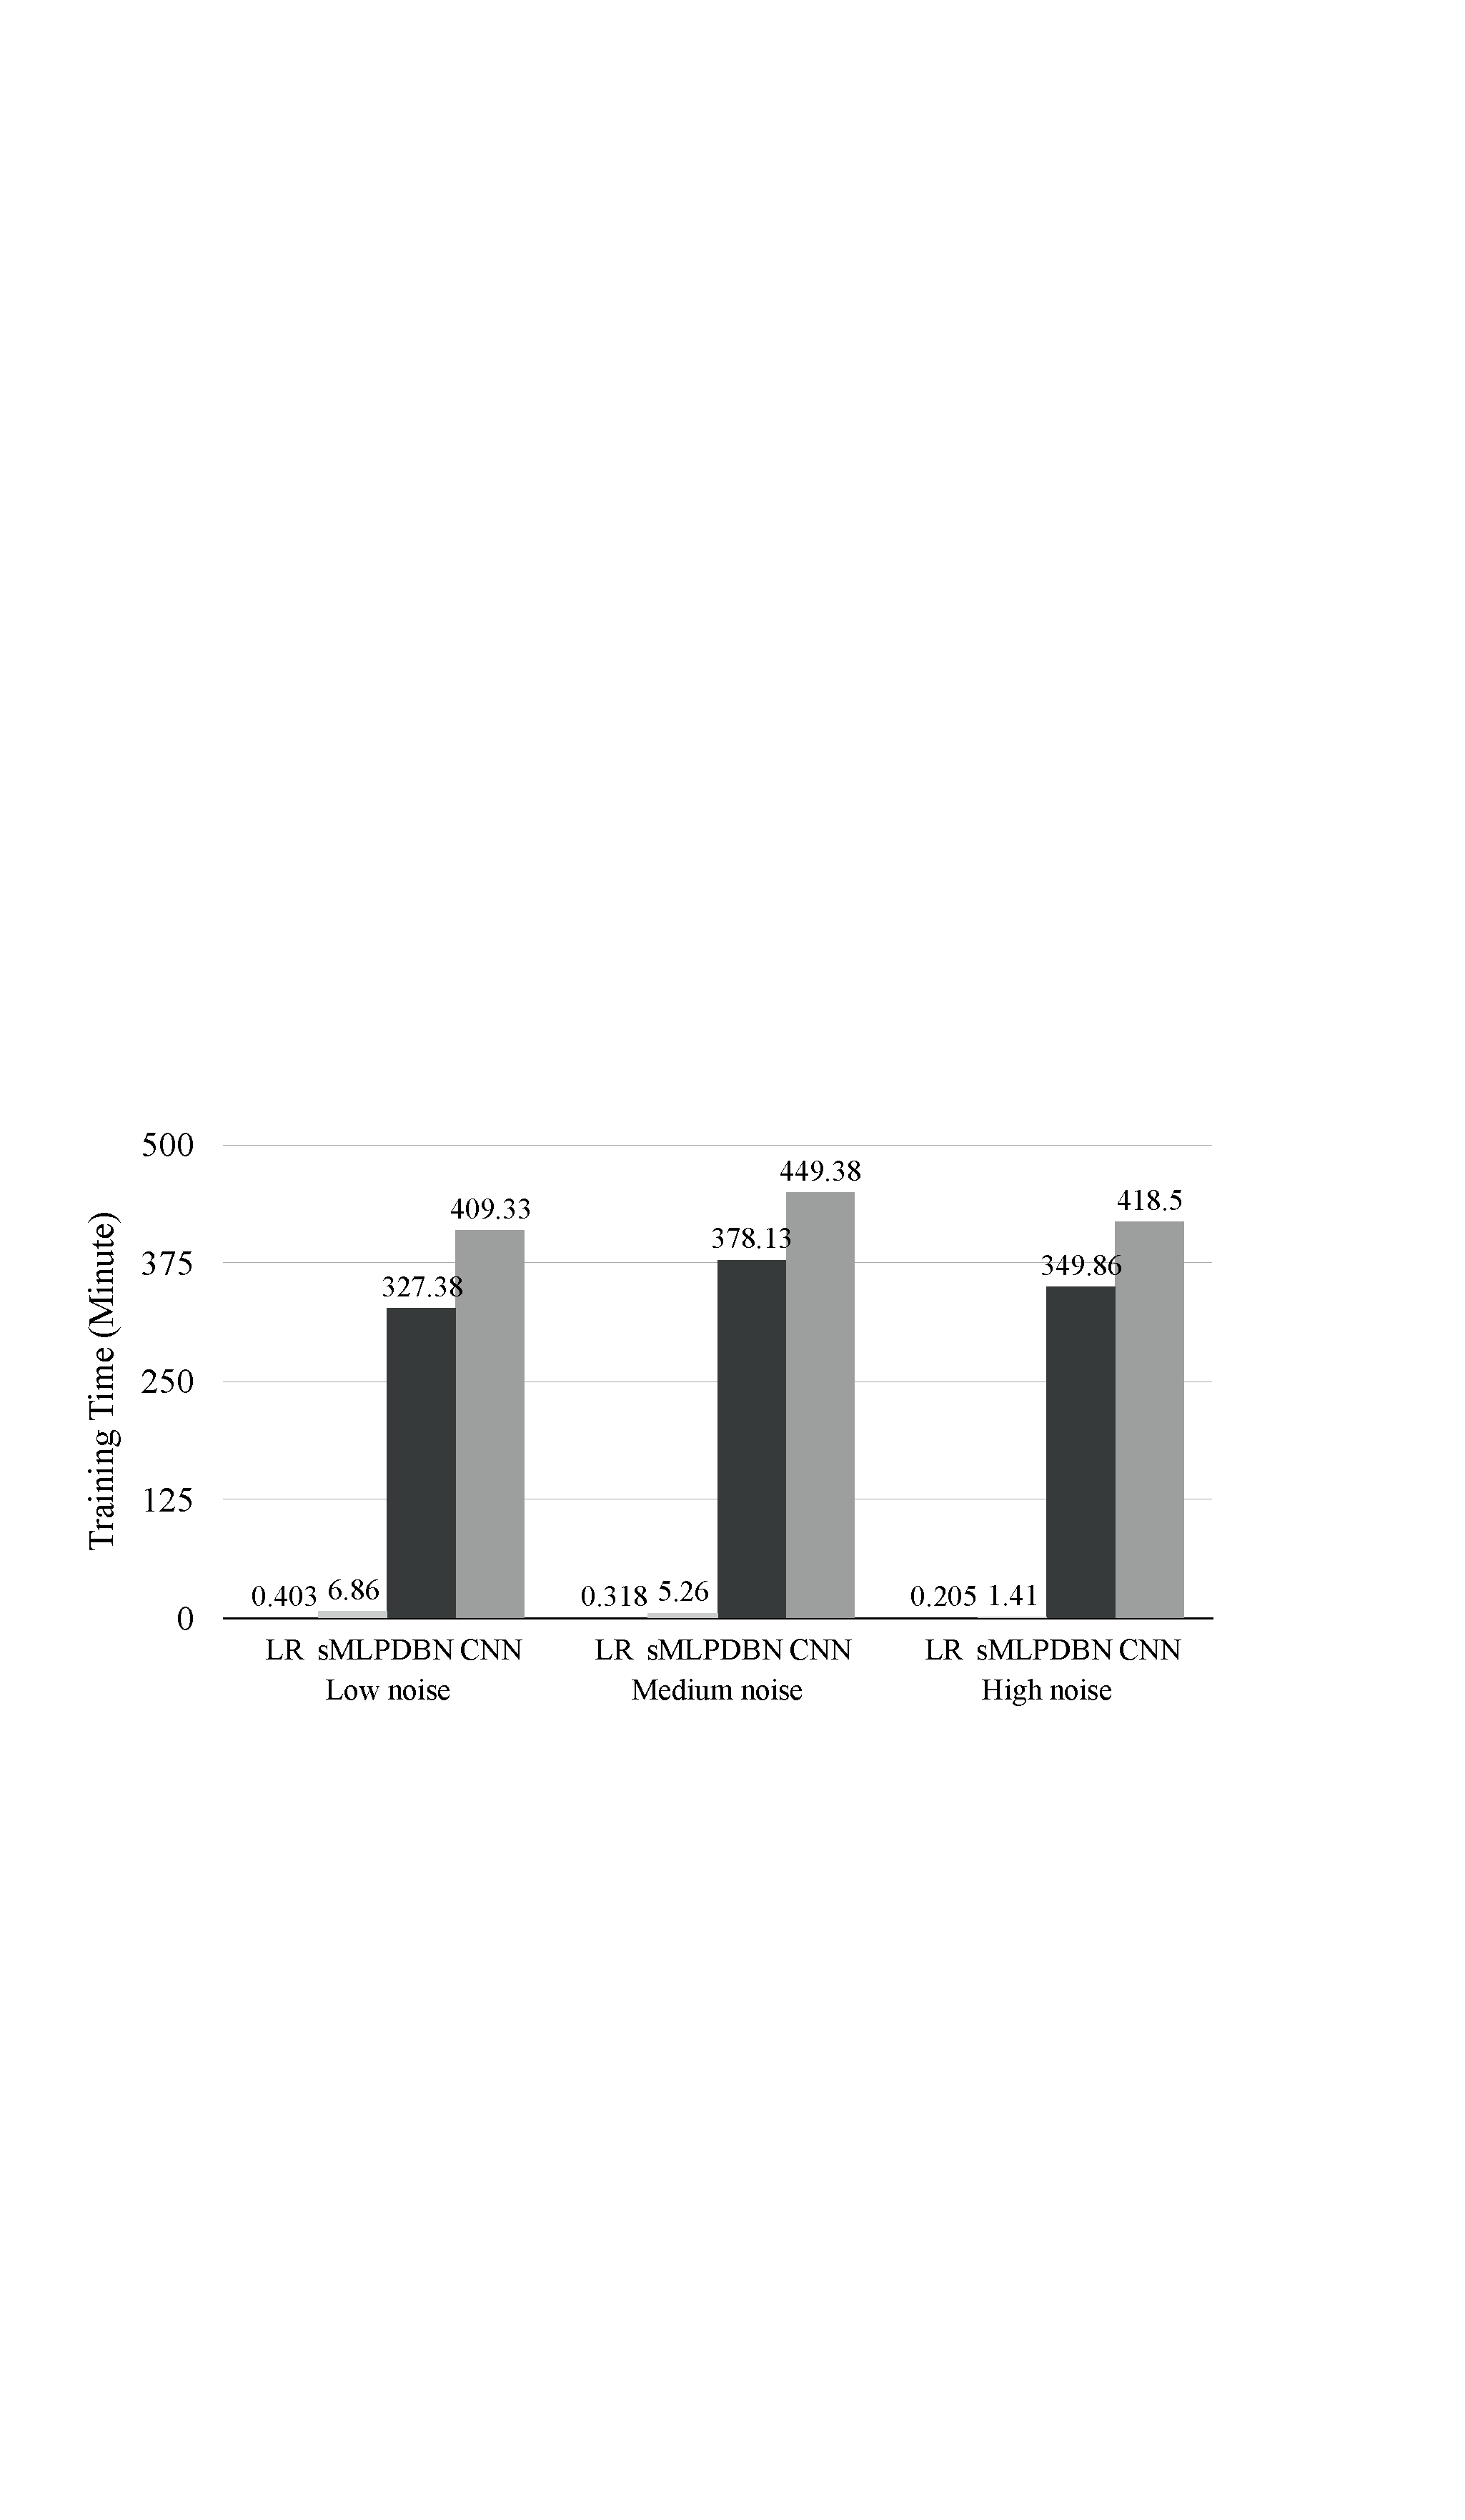
\includegraphics[trim = 0mm 0mm 0mm 12mm,clip,width=3.4in]{figs/t}
	\caption{Training time.} \label{fig:time}
\end{figure}  

 


\section{Request Rate Allocation}\label{sec:rateall}

As shown in Fig.~\ref{fig:sys}, after having been notified of the optimal backend capacity by Clockwork, the developer will purchase a new MBaaS service plan or adjust the instance configuration on Amazon EC2  accordingly. Given the backend capacity fixed for the upcoming hour, there are three potential ways for Clockwork to conduct request scheduling for all users, as shown in Fig.~\ref{fig:sch}. 


\emph{Proxy mode}. As shown in Fig.~\ref{fig:sch}(a), users send all their requests to the cloud servers of Clockwork, which acts as a proxy to redirect these requests to the backend. Given that the backend capacity is $N$, we can simply sort all requests according to their delay tolerance, and send the top $N$ most urgent requests every minute. Nevertheless, an important concern with this approach is privacy. Users are, in general, not willing to reveal sensitive information to a third-party cloud service provider such as Clockwork. For this reason, it is better for users to send requests directly to the backend by themselves, but with scheduling instructions from Clockwork.

\emph{Tight control}. As shown in Fig.~\ref{fig:sch}(b), whenever a new request is generated, instead of sending it to Clockwork, the user informs Clockwork of the type and initiation time of the request, then waits for the permission to send the request to the backend. Similar to the proxy mode, every minute, Clockwork can simply give permissions to the top $N$ most urgent requests. Though this approach avoids the privacy issues, it is not scalable as the frequent communications between users and Clockwork may lead to an excessive amount of overhead and long latencies. 

\emph{Rate allocation}. To overcome the drawbacks of a stringent centralized control mechanism and give users more autonomy, we adopt a rate-based scheduling strategy, as shown in Fig.~\ref{fig:sch}(c). Within each minute, Clockwork periodically assigns rates to users, based on their reported request information. Users then schedule their own requests according to the allocated rates. In the remainder of this section, we derive a rate allocation strategy that is proved to be fair and Pareto-optimal.  

\begin{figure}[t]
	\center
	\hspace{-0cm}
	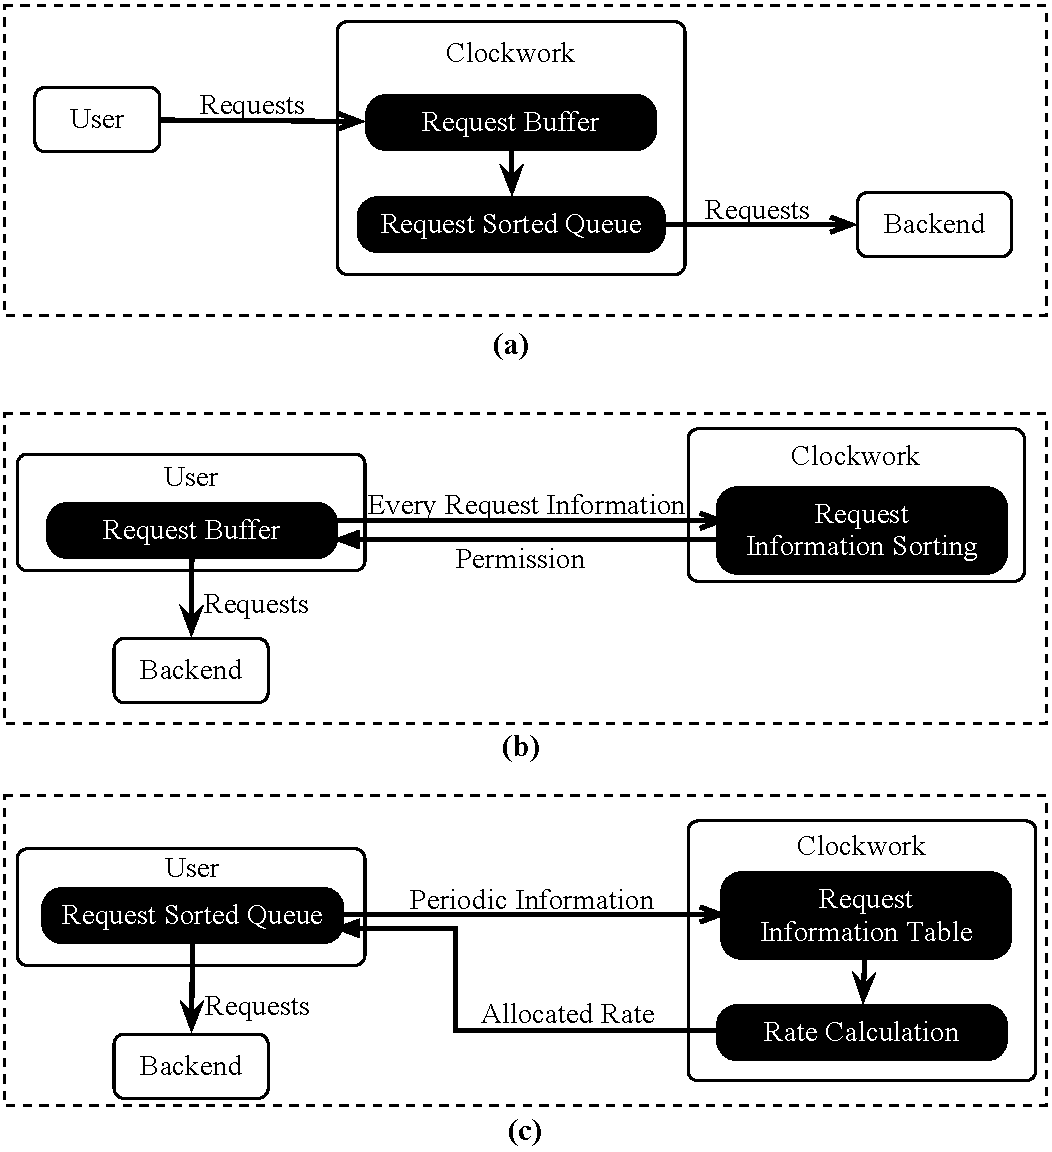
\includegraphics[width=3.2in]{figs/schedule}
	\caption{Three ways of requests scheduling.} \label{fig:sch}
	\vspace{-0.cm}
\end{figure}     

Assume that there is a finite set of $S$ users. We divide each minute into $1,2,...,T$ time slots, and users contact the cloud servers of Clockwork for a new rate at the start of each time slot. Given the backend capacity as $N$, the cap for the number of requests per time slot is $N/T$, shared by all users. At time slot $\tau$, the number of requests of user $s$ is denoted by $X_s(\tau)$, so the overall request state is $\pmb{X}(\tau)=\big(X_1(\tau), \cdots, X_S(\tau)\big)$. Clockwork allocates a rate of $R_s(\tau)$ to user $s$, the maximum number of requests that user $s$ can send within time slot $\tau$. We have $\pmb{R}(\tau) = \big(R_1(\tau),\cdots,R_S(\tau)\big)$. A rate allocation result $\pmb{R}(\tau)$ is feasible if the cap is not hit, that is, $\sum_{s=1}^{S}R_s(\tau) \le N/T$. Leveraging the definition of utility functions of the network utility maximization (NUM) problem \cite{yi2008stochastic}, we assume that the utility of assigning rate $R_s(\tau)$ to user $s$ is $X_s(\tau)\cdot U_s\big(\frac{R_s(\tau)}{X_s(\tau)}\big)$, in which $U_s(\cdot)$ is a function of $\frac{R_s(\tau)}{X_s(\tau)}$. Our objective  is to maximize the weighted sum of utilities of all users.

\begin{align}\label{equ:quota-allocation}
\vspace{-0.5cm}
\max\limits_{R_s(\tau)}~ & \sum_{s=1}^{S} \omega_s(\tau)*X_s(\tau) * U_s\big(\frac{R_s(\tau)}{X_s(\tau)}\big),\nonumber\\
	\textrm{subject to } & \sum_{s=1}^{S}R_s(\tau) \le \frac{N}{T}.
	\end{align}
in which $\omega_s(\tau)$ is the weight of user $s$, specified by the developer. The weight $\omega_s(\tau)$ is added to account for the delay tolerance of requests. If most of the requests of user $s$ are urgent, $\omega_s$ should be larger. To treat all users without bias, we adopt the same utility function for all users, i.e., $U_s(\cdot) = U(\cdot), \forall s$. Utility function $U(\cdot)$ is usually assumed to be non-decreasing and concave \cite{yi2008stochastic}. This is reasonable because a higher rate will naturally lead to a higher utility, and the increment of utility is more significant when the rate is low, but less significant when the rate is already high. We will show that, with a proper utility function $U(\cdot)$, the rate allocation result $\pmb{R}(\tau)$, as the solution to the maximization problem in (\ref{equ:quota-allocation}), can be fair and Pareto-optimal. More specifically, we choose the $\alpha$-fair utility function, widely used in the field of network resource allocation, to help achieve these ideal properties \cite{yi2008stochastic}.
	
	\begin{definition} ($\alpha$-fair function). 
		$\alpha$-fair function, introduced by Mo and Walrand \cite{mo2000fair}, is defined as:

		
		\begin{equation}\label{equ:N_w_2}
		U^{\alpha}(x) = \left\{ \begin{array}{ll}
		\frac{x^{1-\alpha}}{1-\alpha}, &\textrm{for } \alpha \in (0,\infty) \setminus \{1\},   \\
		\log x, &\textrm{for } \alpha = 1. \end{array}  \right.
		\end{equation}
		 
	\end{definition} 
	
	\begin{definition}\label{def:fairallocation}($\alpha$-fair rate allocation). 
		A feasible rate allocation result $\pmb{R}$ is called (weighted) $\alpha$-fair if, for any other feasible rate allocation result $\pmb{R}'$, we have: 
		\begin{equation}
		\sum_{s=1}^{S} w_s\frac{R'_s - R_s}{R_s^{\alpha}} \le 0. 
		\end{equation}
	\end{definition}

$\alpha$-fair rate allocation is equivalent to proportional fair rate allocation when $\alpha \rightarrow 1$, and max-min fair rate allocation when $\alpha \rightarrow \infty$. In the following context, we first give the rate allocation result according to the maximization problem in (\ref{equ:quota-allocation}) with $\alpha$-fair function, then prove that it is $\alpha$-fair and Pareto-optimal. 
	
	\begin{proposition}\label{the:rate}
		At time slot $\tau$, given the request state $\pmb{X}(\tau)$ and the cap of the number of requests  $N/T$, the rate allocation result based on $\alpha$-fair function is:
		
		\begin{equation}\label{equ:allocation}
		R_s^*(\tau) = \frac{(\omega_s(\tau))^{1/\alpha} X_s(\tau) }{\sum_{s=1}^S (\omega_s(\tau))^{1/\alpha} X_s(\tau)}\cdot\frac{N}{T}, \forall s. 
		\end{equation} 
	\end{proposition}
	
	\begin{proof}
		The Lagrangian for the problem is given by:  
		\begin{displaymath}
		L(\pmb{R}, \mu) = \sum_{s=1}^S \frac{\omega_s(\tau) X_s(\tau)}{1-\alpha}\big(\frac{R_s(\tau)}{X_s(\tau)}\big)^{1-\alpha} + \mu(\frac{N}{T}-\sum_{s=1}^S R_s(\tau)).
		\end{displaymath}
		The optimal solution corresponds to the stationary point of the Lagrangian function:
		\begin{equation}\label{equ:la}
		\begin{split}
		\frac{\partial L}{\partial R_s(\tau)} &= \omega_s(\tau)(\frac{R_s(\tau)}{X_s(\tau)})^{-\alpha} - \mu, \forall s,\\
		\frac{\partial L}{\partial \mu}& = \frac{N}{T} -\sum_{s=1}^{S} R_s(\tau).
		\end{split}
		\end{equation}
		By setting $\partial L /\partial R_s(\tau) = 0$, we have:
		\begin{equation}\label{equ:1}
		R_s(\tau) = X_s(\tau) (\frac{\mu}{\omega_s(\tau)})^{-\frac{1}{\alpha}}, \forall s.
		\end{equation}
		By setting $\partial L /\partial \mu = 0$, we have:
		\begin{equation}\label{equ:2}
		\sum_{s=1}^SR_s(\tau) = \frac{N}{T} = \sum_{s=1}^SX_s(\tau) (\frac{\mu}{\omega_s(\tau)})^{-\frac{1}{\alpha}}.
		\end{equation}
		Combining (\ref{equ:1}) and (\ref{equ:2}), we can get the rate allocation result as (\ref{equ:allocation}). 
	\end{proof}
	
	\begin{theorem}
		The rate allocation result given by Proposition \ref{the:rate} is weighted $\alpha$-fair.  
	\end{theorem}
	
	\begin{proof}
    Let $\pmb{R}(\tau) \ne \pmb{R}^*(\tau)$ denote an arbitrary feasible rate allocation result. Multiplying  (\ref{equ:1}) by $(R_s(\tau) - R_s^*(\tau))$, we have:
    \begin{displaymath}
    \big(R_s(\tau) - R_s^*(\tau)\big)\omega_s(\tau) \big(\frac{R_s^*(\tau)}{X_s(\tau)}\big)^{-\alpha} = \mu \big(R_s(\tau) - R_s^*(\tau)\big).
    \end{displaymath} 
    Summing over all $s$, we have:
    \begin{displaymath}
    \sum_{s=1}^S\omega_s(\tau) X_s(\tau)\frac{R_s(\tau) - R_s^*(\tau)}{(R_s^*(\tau))^{\alpha}}  = \mu \sum_{s=1}^S\big(R_s(\tau) - R_s^*(\tau)\big).
    \end{displaymath} 
     According to (\ref{equ:la}), we have $\sum_{s=1}^{S} R_s^*(\tau) = {N}/{T}$ and
     
     \noindent$\sum_{s=1}^{S} R_s(\tau) \le {N}/{T}$. Hence, we have:
     \begin{displaymath}
     \begin{split}
     \sum_{s=1}^S\omega_s(\tau) X_s(\tau)&\frac{R_s(\tau) - R_s^*(\tau)}{(R_s^*(\tau))^{\alpha}} = \mu \sum_{s=1}^S\big(R_s(\tau) - R_s^*(\tau)\big) \\
     &= \mu (\sum_{s = 1}^S R_s(\tau) -\sum_{s=1}^S R_s^*(\tau)) \le 0.
     \end{split}
     \end{displaymath}
     The strict inequality holds for all $\pmb{R}(\tau)\ne \pmb{R}^*(\tau)$, due to the uniqueness of $\pmb{R}^*(\tau)$. Based on definition \ref{def:fairallocation}, the rate allocation result given by (\ref{equ:allocation}) is weighted $\alpha$-fair.  
	\end{proof}
	
	The efficiency of the rate allocation result given by Theorem \ref{the:rate} is characterized by Pareto-optimality as follows. 
	
	\begin{definition}(Pareto-optimality). A rate allocation result $\pmb{R}(\tau)$ is said to be Pareto-optimal, if for any rate allocation result $\pmb{R}'(\tau)$, which satisfies $\forall s, R_s'(\tau) \ge R_s(\tau)$,  it must be true that $\pmb{R}(\tau) = \pmb{R}'(\tau)$. 
	\end{definition}
	
	Pareto-optimality implies that there is no other rate allocation result that can improve every user's utility by assigning everyone a higher rate. 
	
	\begin{theorem}
		The rate allocation result given by Proposition \ref{the:rate} is Pareto-optimal.  
	\end{theorem} 
	\begin{proof}
		Assume that there exists a feasible rate allocation result $\pmb{R}(\tau)$, which satisfies $\forall s, R_s(\tau) \ge R_s^*(\tau)$. We have:
		\begin{displaymath}
		\begin{split}
		&\sum\limits_{s=1}^S R_s(\tau) \ge \sum\limits_{s=1}^S R_s^*(\tau) \\
		&= \sum\limits_{s=1}^S\frac{(\omega_s(\tau))^{1/\alpha} X_s(\tau) }{\sum_{s=1}^S (\omega_s(\tau))^{1/\alpha} X_s(\tau)}\cdot\frac{N}{T} =\frac{N}{T}.
		\end{split}
		\end{displaymath}
		If $\pmb{R}(\tau) \ne \pmb{R}^*(\tau)$, there exists at least one user $s$, $R_s(\tau) > R_s^*(\tau)$, and the cap on the number of requests per time slot will be violated. Therefore, it must be true that $\pmb{R}(\tau) =\pmb{R}^*(\tau)$. 
	\end{proof}

  	




	
	
	

\section{System Implementation} \label{sec:implementation}

In this section, we first discuss implementation issues regarding the computation of rate allocation on the cloud servers. Then, we address the problem of request scheduling on user devices.


\subsection{Rate Computation on Cloud Servers}

\subsubsection{User Synchronization}

In our implementation, we set the number of time slots within a minute as $T = 4$, i.e., users report their request information to cloud servers of Clockwork and obtain the allocated rate every $15$ seconds. Three kinds of HTTP requests are used for users to communicate with cloud servers. The first kind of HTTP requests are sent when users launch the application or restart the application from background. The cloud servers will reply with an initial rate $R_0$ and the synchronization reference. $R_0$ is above zero, since we find that upon logging in, users tend to perform many operations, thus sending many requests. If $R_0=0$, these requests can not be sent until a new rate is assigned at the next time slot, which may lead to a poor user experience.
 

The second kind of HTTP requests are used to periodically report users' request information and ask for rate allocation. The cloud servers maintain a table of all active users, including the user ID, number of requests $\pmb{X}(\tau)$, weight $\pmb{\omega}(\tau)$, and the rate allocation result $\pmb{R}(\tau)$. Users log in at different times, and the local time on their mobile devices may be different from the time on cloud servers. We need to synchronize users to ensure that they update $\pmb{X}(\tau)$ and $\pmb{\omega}(\tau)$ at (almost) the same time for cloud servers to compute the rate allocation $\pmb{R}(\tau)$. Recall that the response to the first kind of HTTP requests upon user arrival includes a synchronization reference. We use the \emph{second} of the server time as this synchronization reference. For example, if a new user arrives at \formattime{00}{00}{43} of the server time, the synchronization reference will be $43$, which is then fed into a (one-time) \emph{timer} function on the user device. The function will be executed after $15-(43\mod 15) = 2$ seconds, i.e., at \formattime{00}{00}{45} of the server time, triggering another (iterative) \emph{timer} function that will communicate with the cloud servers every $15$ seconds. In this way, all users will be synchronized to report their request information at the start of each time slot.

The last kind of HTTP requests are used to inform the cloud servers that the application goes to background or is terminated, so that the user will be removed from the rate allocation table. 

If a user's HTTP requests fail, the application will get an error message. In this case, without allocated rate from the cloud servers, the user device will carry out a default request scheduling mechanism, which we will describe in Section \ref{sec:default}). Meanwhile, the user will keep trying to contact the cloud servers every $15$ seconds.   

\subsubsection{Rate Allocation Computation}\label{sec:rate}

We classify all requests into $K = 3$ types: type $3$ requests are the most urgent, and type $1$ requests are the least urgent. Then we define that the weight of a user is the sum of types of all her requests. For example, if user $s$ has 15 type 1 requests, 10 type 2 requests, and 5 type 3 requests, her weight is $\omega_s(\tau) = 15*1+10*2+5*3 = 50$.  It can be easily checked that a user with more urgent requests will get a higher weight.

Since users will turn up for new rates at the start of time slot $\tau+1$, the cloud servers need to calculate the rate allocation result $\pmb{R}(\tau+1)$ before the end of time slot $\tau$, by which the reports on $\pmb{X}(\tau)$ and $\pmb{\omega}(\tau)$ haven't been submitted yet. One option is for the cloud servers to wait for $\pmb{X}(\tau)$ and $\pmb{\omega}(\tau)$ at the beginning of time slot $\tau+1$, and then compute $\pmb{R}(\tau+1)$ accordingly. However, users' HTTP requests will not arrive at exactly the same time, due to different network conditions. Early users may have to wait an undesirably long time for all other users to report their information, after which the new rate allocation can be calculated. To avoid this situation, we decide that the cloud servers will work out the new rate allocation $\pmb{R}(\tau+1)$ $5$ seconds before the end of each time slot, using the available information $\pmb{X}(\tau-1)$ and $\pmb{\omega}(\tau-1)$. 


\subsubsection{Request Cap Adjustment}      

When computing rate allocation for each time slot, we assume that the cap on the number of requests to be sent is $N/T$, in which $N$ is the backend capacity, and $T$ is the number of time slots within a minute. However, as some of the allocated rates may be unused (as $X_s(\tau) < R_s(\tau)$), we can adjust the cap to make a better use of the backend capacity. At the first time slot of each minute, the cap will be $N/T$; at the following time slots, the cap will be $N/T$ plus the remaining rates from the previous time slot. For example, if the backend capacity is $1800$, and each minute is divided into $T=4$ time slots. At time slot $1$, the request cap is $1800/4 = 450$. If the actual number of requests sent to the backend during time slot $1$ is $430$, the request cap at time slot $2$ will be $450+(450-430) = 470$.

 

\subsection{Request Scheduling on User Devices}\label{sec:sending}

\subsubsection{Dynamic Request Scheduling}
The user device will keep a queue of requests ranked in a non-ascending order of priorities that are jointly determined by the type and the initiation time of a request. A new request will be inserted into the queue, and wait for its turn to be sent to the backend. Let $\pmb{Q}_s(\tau) = (q_{s,1}(\tau), q_{s,2}(\tau),\cdots)$ denote the request queue of user $s$, in which $q_{s,i}(\tau)$ is the priority of the $i$-th request, and we have $q_{s,1}(\tau) \ge q_{s,2}(\tau)\ge \cdots$. The number of requests in the queue is denoted by $|\pmb{Q}_s(\tau)|$.

A major problem facing the request scheduling on the user device is that the new rate obtained at the start of a time slot may not be able to cater to the new requests arrived later during the time slot. More specifically, at the start of time slot $\tau$, upon receiving a new rate $R_s(\tau)$, if user $s$ instantly sends the top $R_s(\tau)$ requests in the queue $\pmb{Q}_s(\tau-1)$ (given that $|\pmb{Q}_s(\tau-1)| > R_s(\tau)$), an urgent request generated later during time slot $\tau$ can no longer be sent. For example, at \formattime{00}{00}{15}, with a queue of $(2,1,1)$ and an allocated rate of $2$, the user device sends the first $2$ requests in the queue right away to the backend. At \formattime{00}{00}{25}, a new request with a priority of $3$ is generated, but has to be detained as the allocated rate is drained. 

The above-mentioned problem arises as the user device can not predict future request dynamics and preserve enough rate for them. To mitigate this problem, we design a threshold-based request scheduling mechanism that works as follows. Firstly, we set a priority threshold $\theta_q$. At the beginning of time slot $\tau$, with the new rate $R_s(\tau)$, user $s$ will immediately send the requests whose priority exceeds $\theta_q$ to the backend. If the number of such requests is greater than $R_s(\tau)$, the first $R_s(\tau)$ will be sent; otherwise, the rest of the rate is reserved for later requests with high priorities. If a newly-generated request has a priority lower than $\theta_q$, it will be inserted in the queue; otherwise, it will be checked whether the allocated rate is exhausted. If yes, the request will be inserted in the queue; otherwise, it will be sent at once to the backend (note that in this case, the queue only contains requests whose priority is lower than $\theta_q$). At the end of time slot $\tau$, if the remaining rate is greater than zero, the user device will send as many queued requests as possible, before asking for a new rate.

\subsubsection{Default Request Scheduling}\label{sec:default}

If the user device fails to get responses from cloud servers of Clockwork, either upon logging in or during periodic rate allocation, a default request scheduling mechanism based on the Additive Increase Multiplicative Decrease (AIMD) algorithm, will come into effect. The requests will be sent to the backend at a lower rate if it is inferred that the current overall request demand is high, vice versa. There are various indications of the current request demand. For example, when using MBaaS, if the request limit is hit, further requests will be rejected with an error message of error code 155. If a user receives such an error message, she should multiplicatively decrease the rate by $b$; otherwise, she will additively increase the rate by $a$: 

\begin{equation}\label{equ:default}
R_s(\tau)= \left\{
\begin{array}{ll}
R_s(\tau-1)+a, &\textrm{if no error code},\\
R_s(\tau-1)/b, &\textrm{if error code}.
\end{array}
\right.
\end{equation}
The default request scheduling will continue until the user device succeeds in getting new allocated rate from cloud servers of Clockwork.


\section{Performance Evaluation}\label{sec:experiment}

\subsection{Experimental Result}

We have developed the client-side of Clockwork as a third-party framework (library) that can be readily used by mobile application developers, using Swift on the iOS platform as a proof-of-concept.  It is implemented using Java on the Amazon Web Service (AWS) platform. For the purpose of our real-world experiments, we have also developed a social messaging iOS application, using Facebook Parse (an MBaaS platform) as its backend, supported by our third-party framework. We identify $17$ different kinds of requests, such as \emph{send a message, send friend request, change username} and so on. We divide them into $K = 3$ types: type $3$ requests are the most urgent and type $1$ requests are the most delay-tolerant. 

To evaluate the performance of Clockwork, we carried out a pilot trial with $15$ iPhone users. We collected data for $20$ hours. Only the statistics regarding the request demand are logged, but not message contents, in order to protect user privacy.

\begin{figure}[t]
	\centering
	\hspace{-0.5cm}
	\begin{minipage}[t]{1.8in}
		\centering
		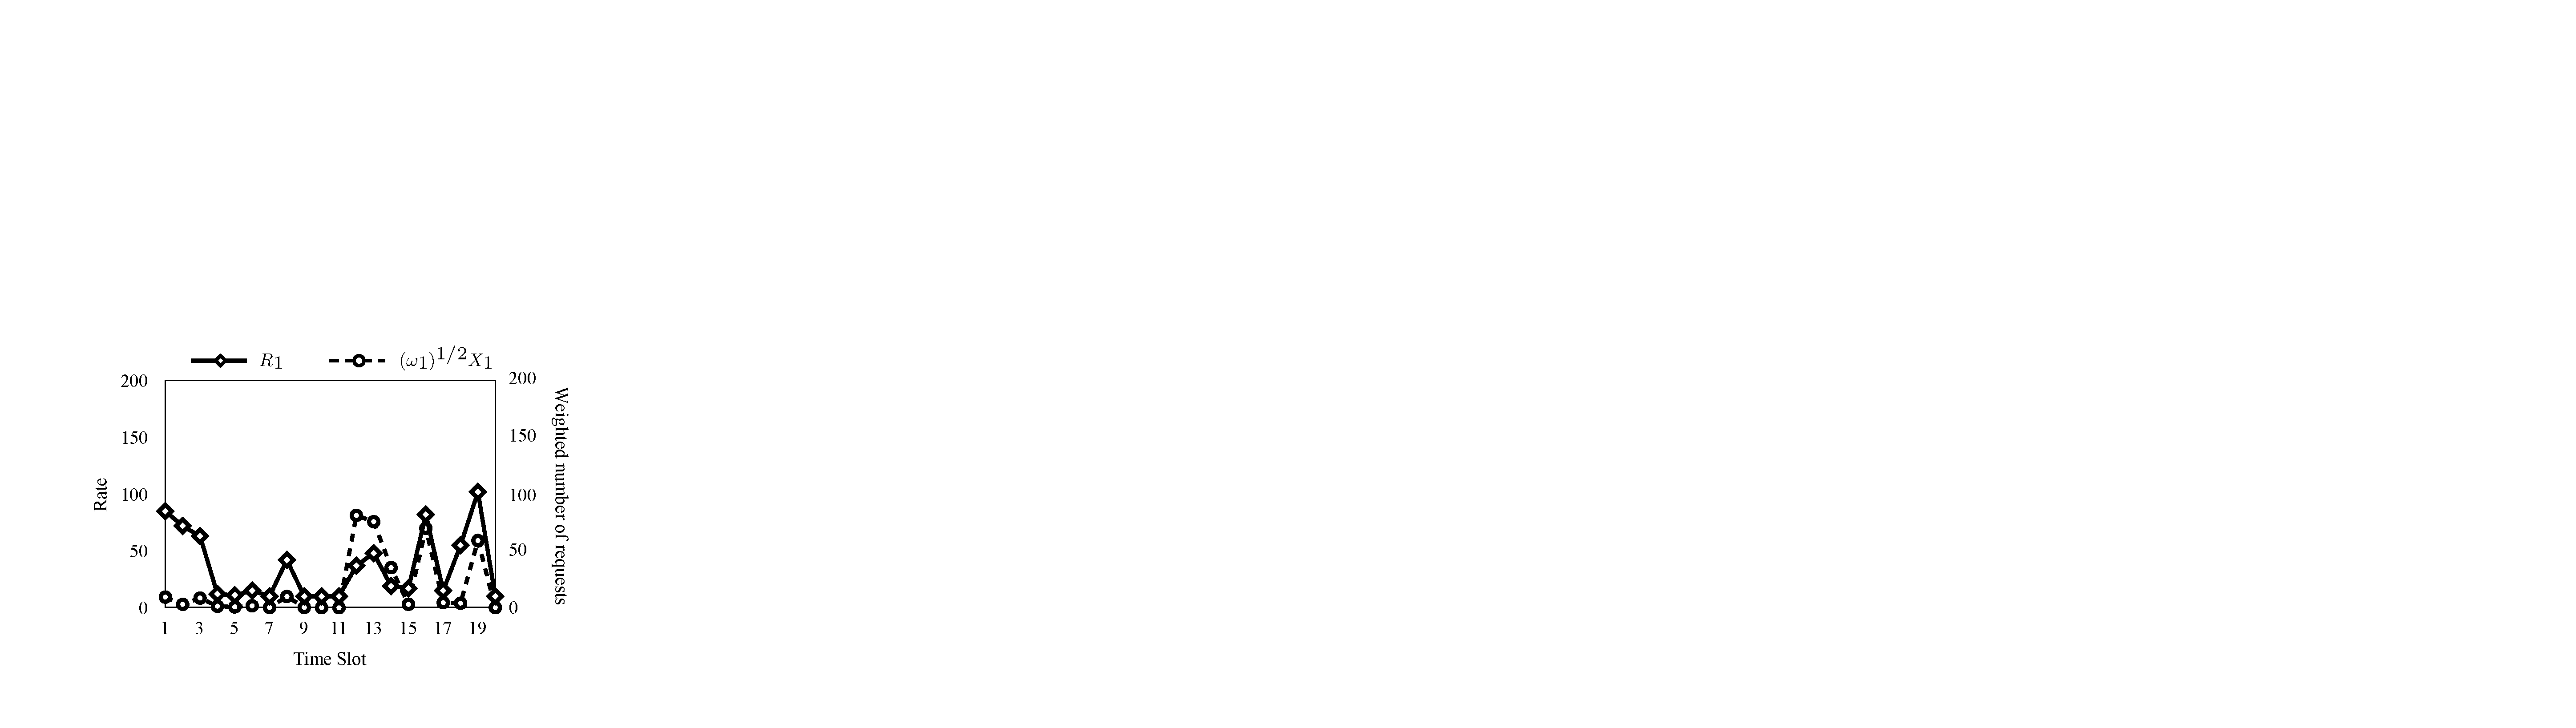
\includegraphics[trim=0mm 0mm 0mm 0mm, clip,width=1.8in]{figs/data1}\\
		\centerline{\small{(a) User 1}}
	\end{minipage}
	\hspace{-0.2cm}
	\begin{minipage}[t]{1.8in}
		\centering
		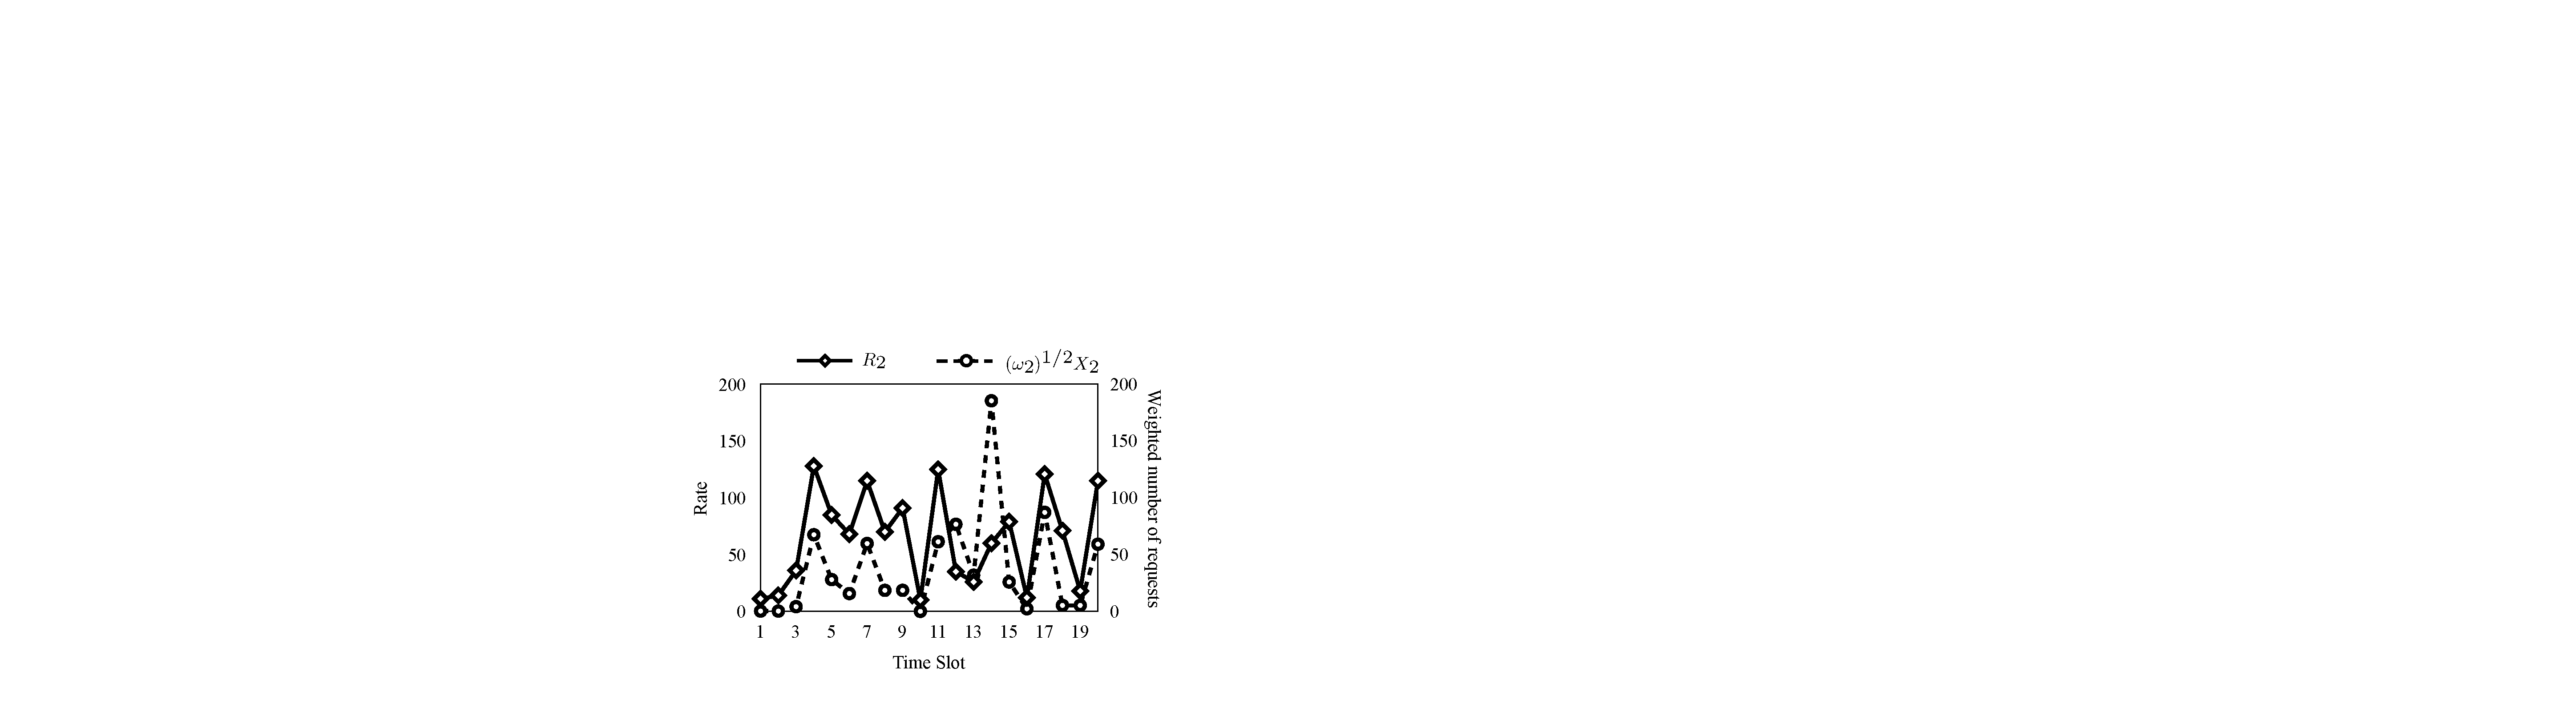
\includegraphics[trim=0mm 0mm 0mm 0mm, clip,width=1.8in]{figs/data2}\\
		\centerline{\small{(b) User 2}}
	\end{minipage}
	\caption{Experimental result of rate allocation.} \label{fig:data}
\end{figure}

 \begin{figure}[t]
	\centering
	\hspace{-0.5cm}
	\begin{minipage}[t]{1.8in}
		\centering
		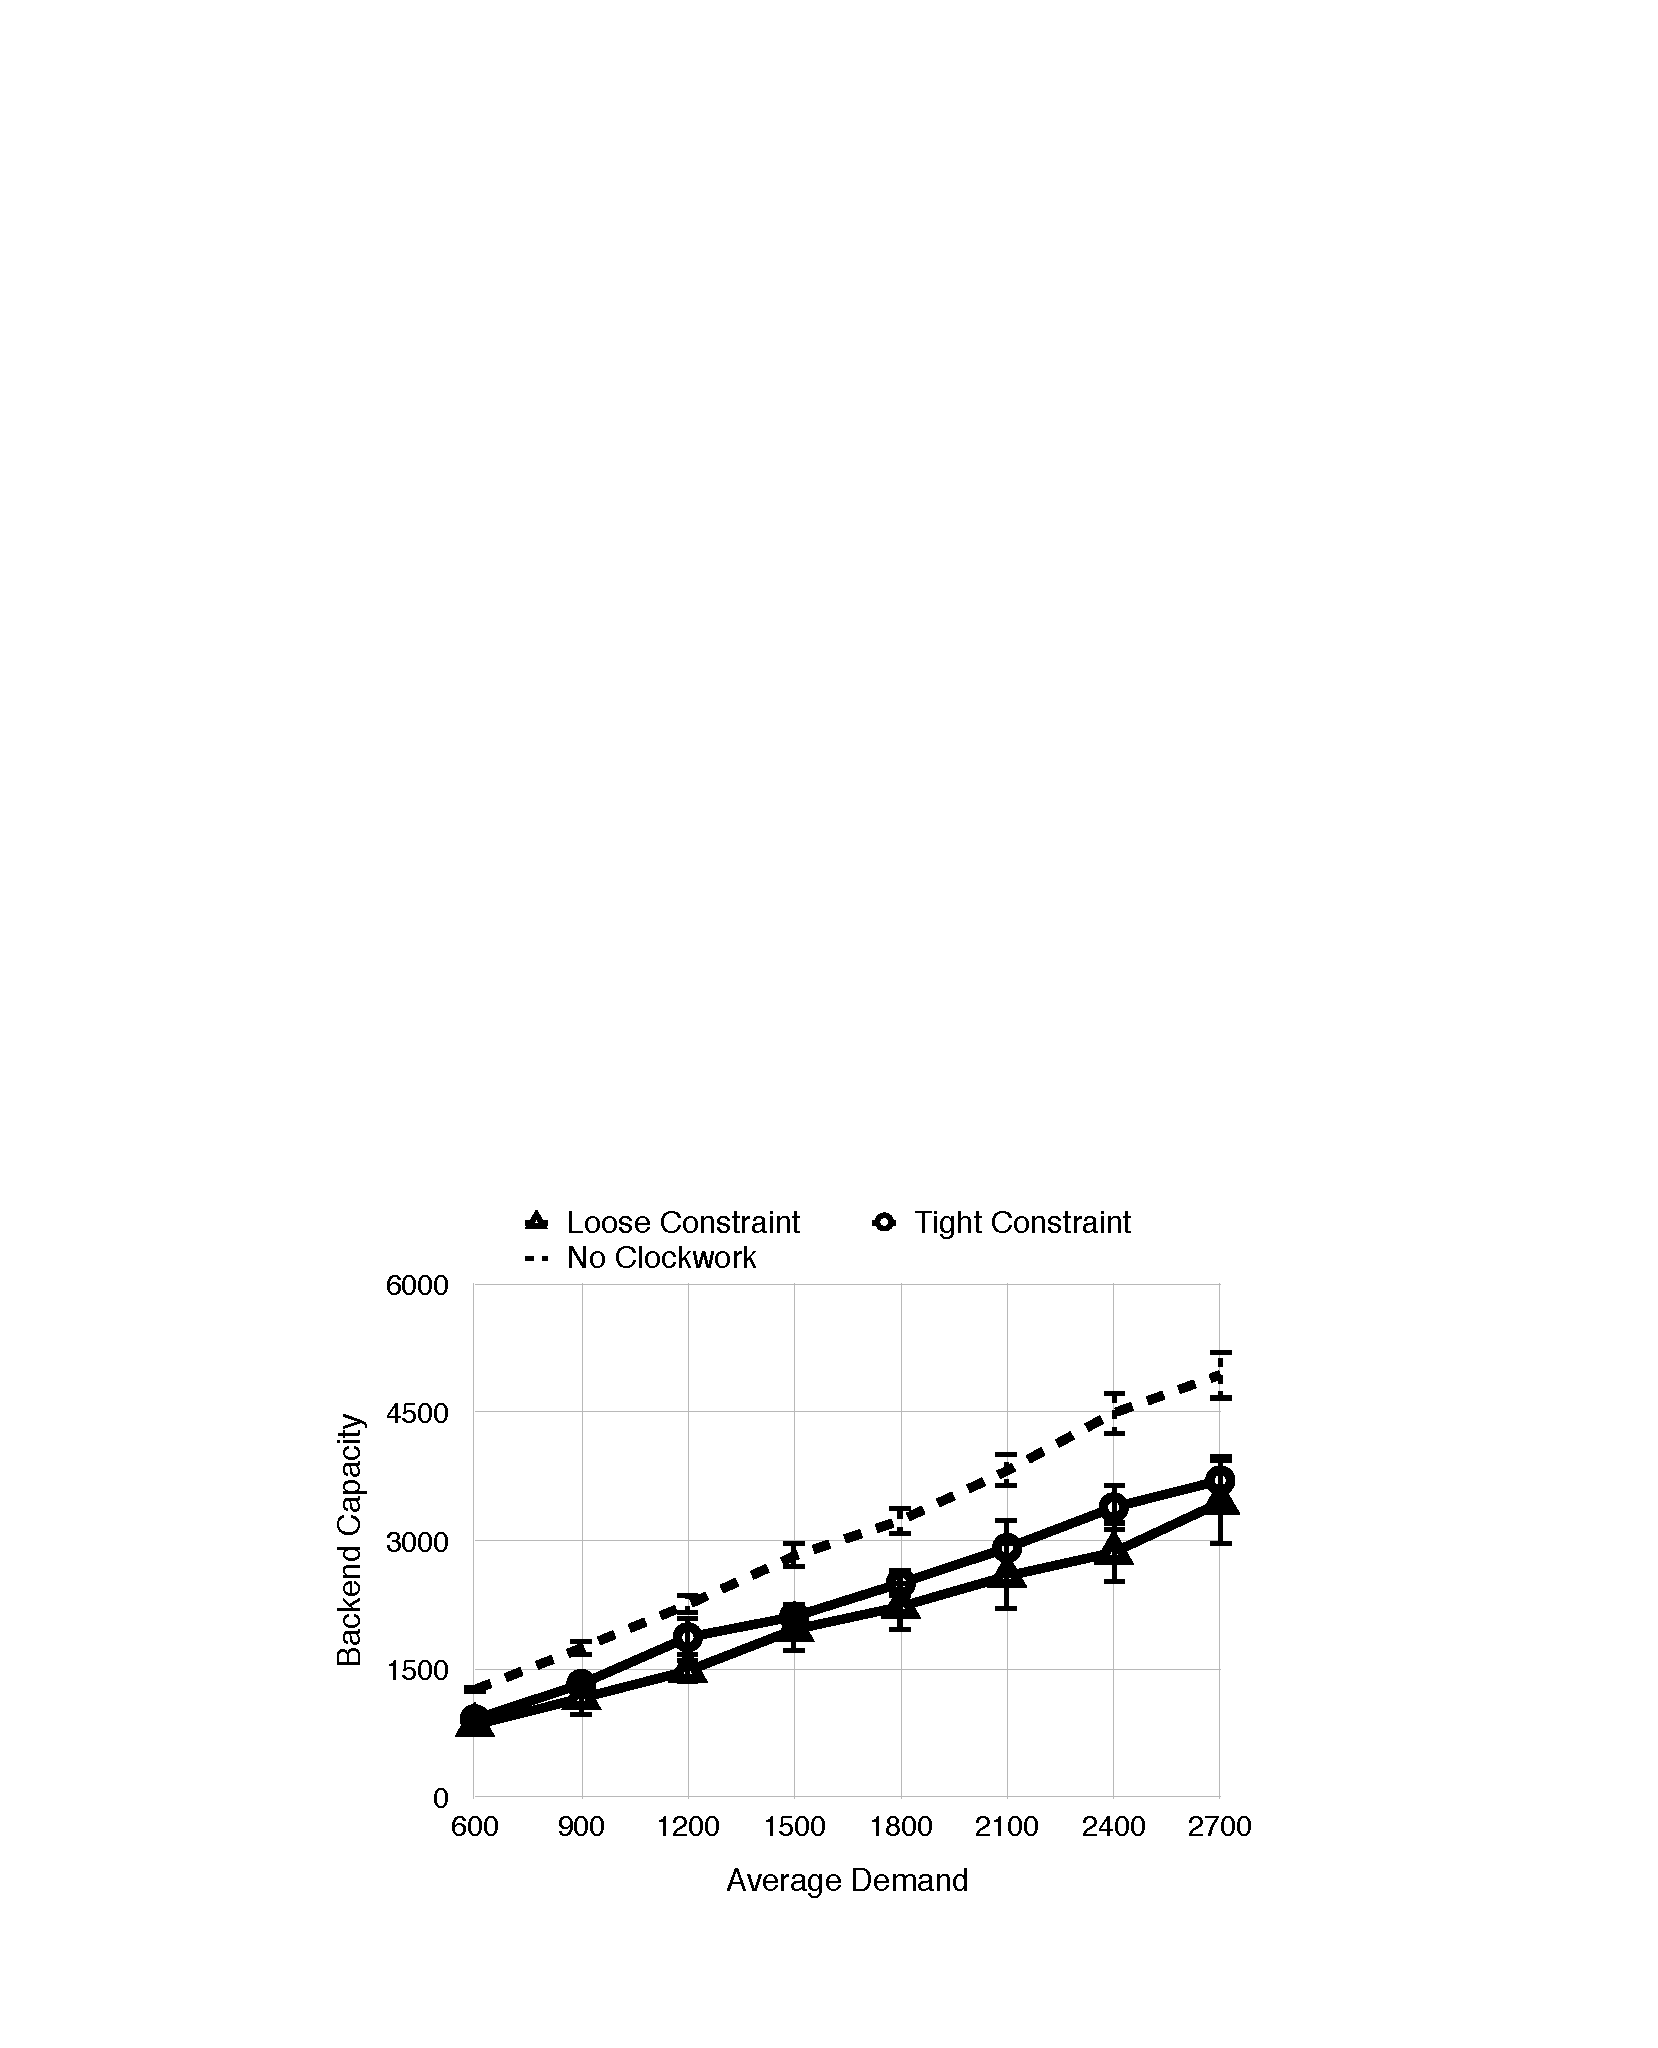
\includegraphics[trim=0mm 0mm 0mm 0mm, clip,width=1.8in]{figs/cp}\\
		\centerline{\small{(a) Required backend capacity}}
	\end{minipage}
	\hspace{-0.2cm}
	\begin{minipage}[t]{1.8in}
		\centering
		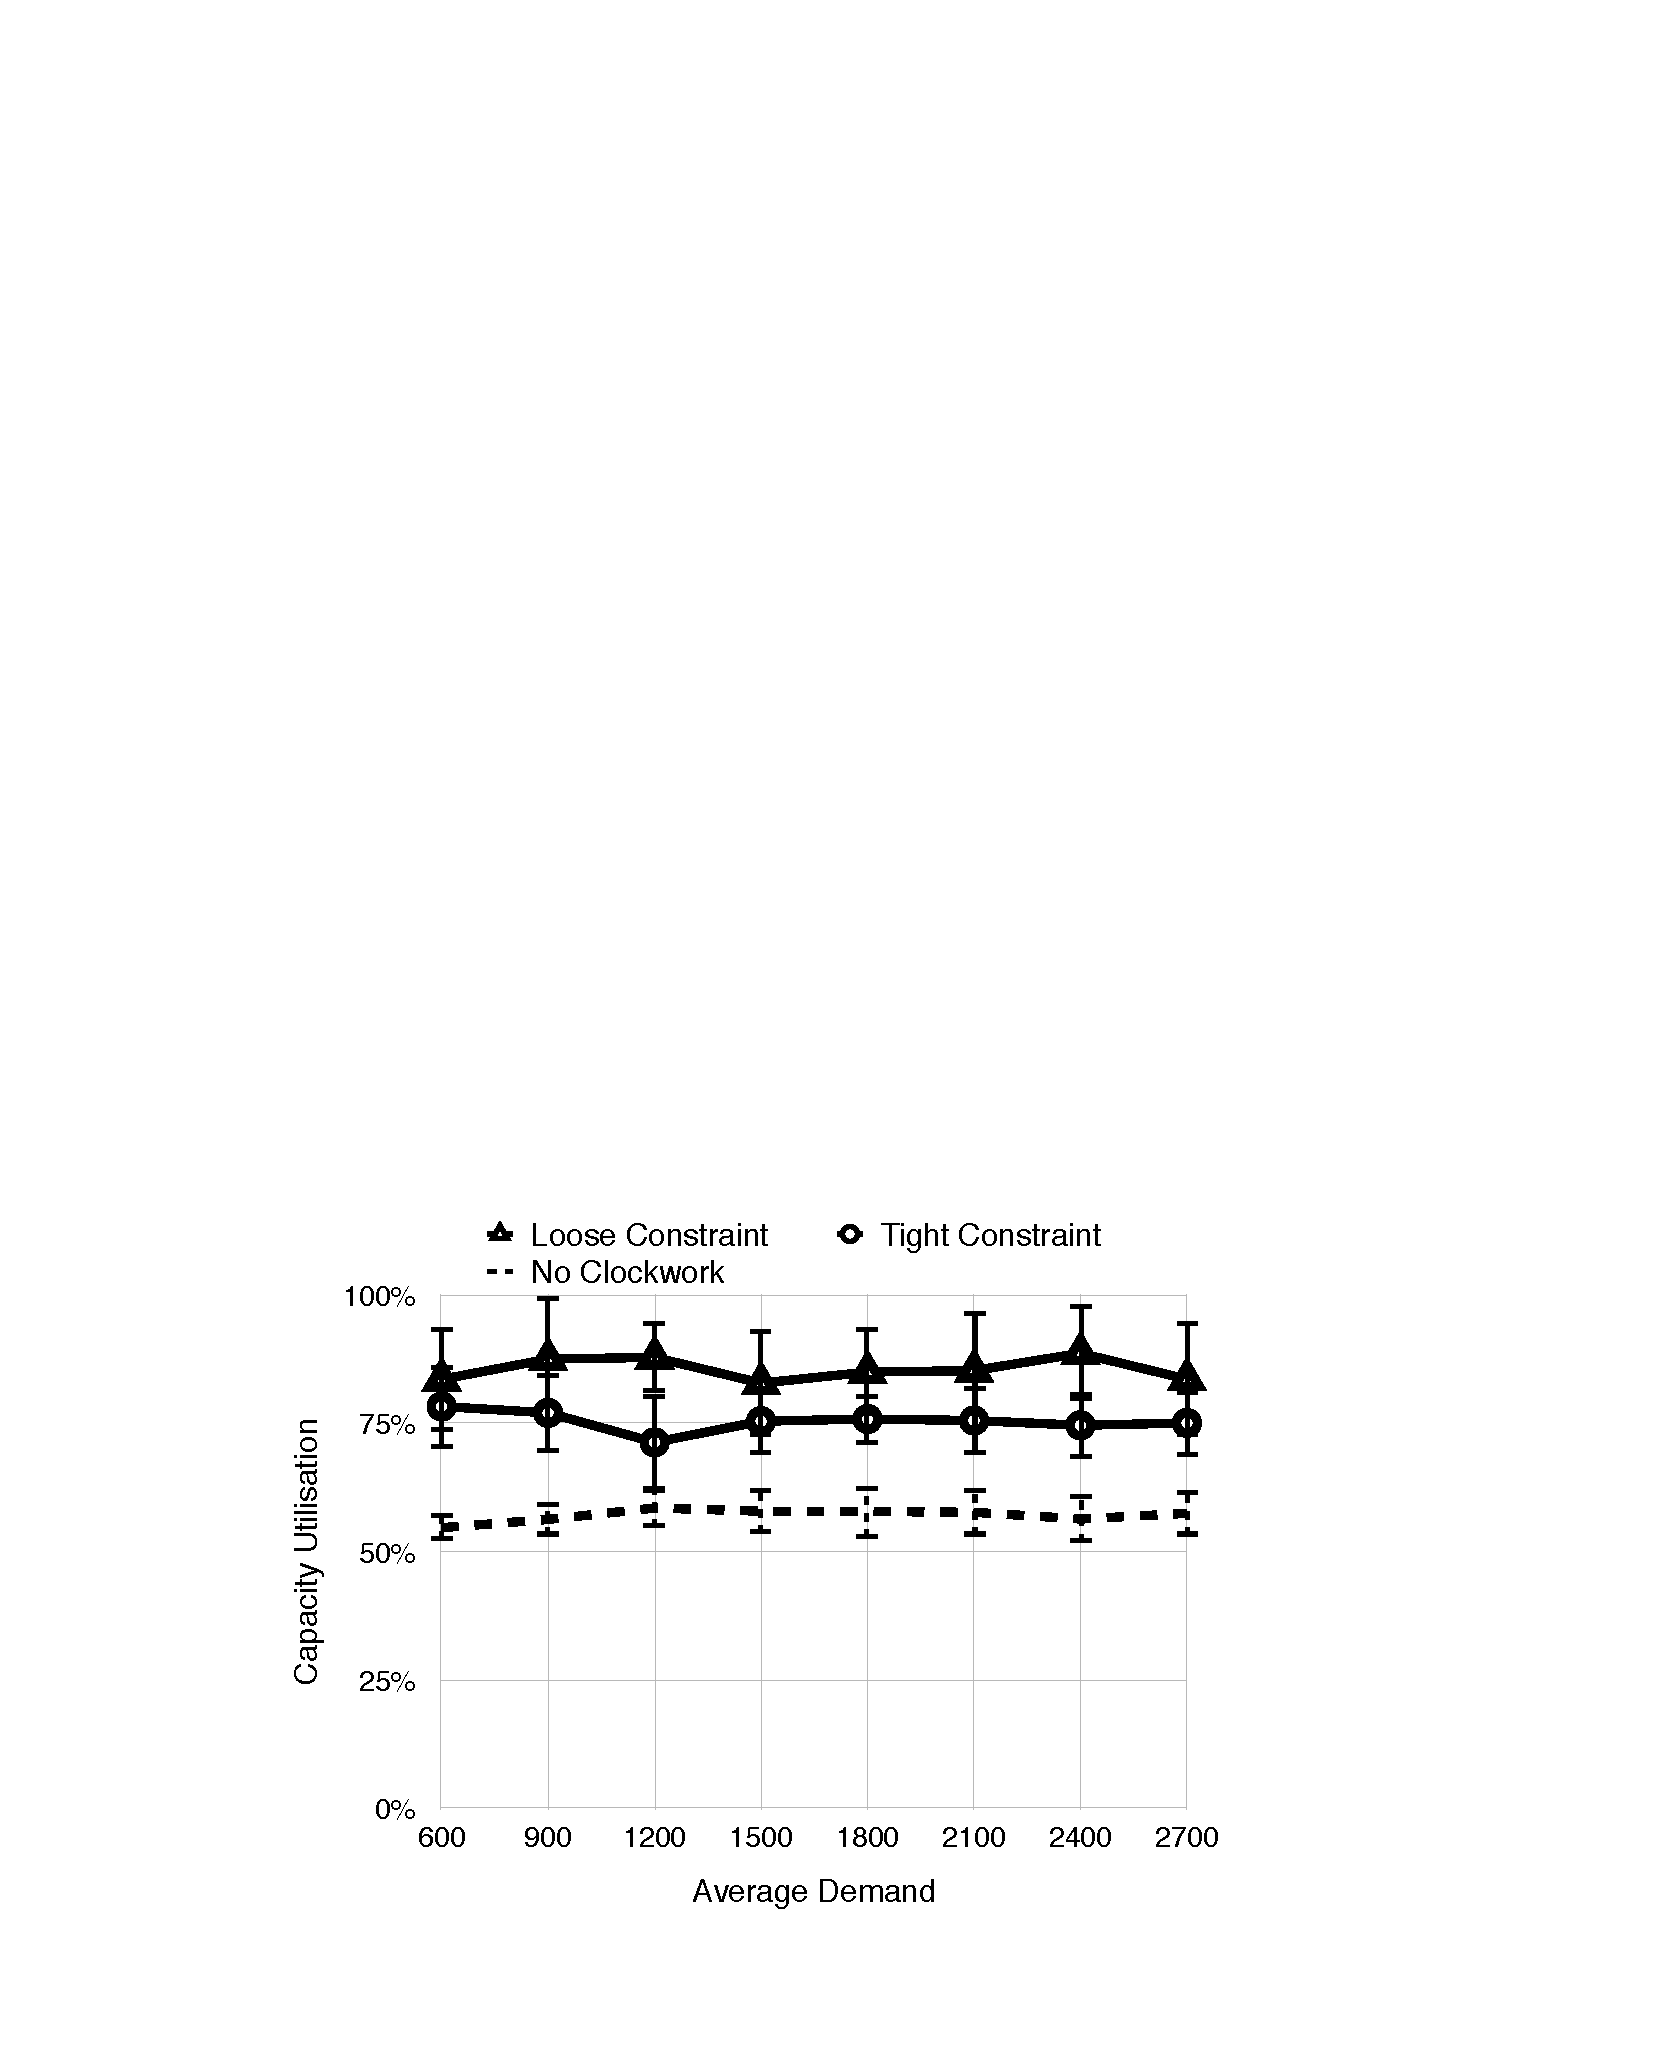
\includegraphics[trim=0mm 0mm 0mm 0mm, clip,width=1.8in]{figs/up}\\
		\centerline{\small{Backend capacity utilization}}
	\end{minipage}
	\caption{Simulation result of backend capacity planning.} \label{fig:serviceplan}
	\vspace{-1cm}
\end{figure}

\emph{Rate allocation}. We set $\alpha = 2$ in the $\alpha-$fair utility function, and show the rate allocation results of two users in Fig.~\ref{fig:data}. Generally speaking, a user will achieve a higher rate if her weighted number of requests is larger. Nevertheless, the allocated rate of a user also depends on the request demand of other users. For example, there is a plunge in user 1's request demand at time slot $15$, but the allocated rate is almost the same as that of the previous time slot. This is because the request demand of user 2 also falls dramatically at time slot $15$, making the ratio of the two users' request demand (i.e., $\frac{(\omega_1)^{1/2} X_1}{(\omega_2)^{1/2} X_2}$) in time slot $15$ approximately the same as that in time slot $14$. Thus, at time slot $15$, each user is assigned a rate similar to that in the previous time slot.

\emph{Capacity planning}. We use the collected data trace as inputs to the optimization problem (\ref{equ:opt}). We compare Clockwork and the baseline, where the backend capacity equals the peak demand. The backend utilization is calculated as the ratio of the average request demand to the backend capacity. The results are shown in Table~\ref{tab:exp}. With Clockwork, the backend cost for the developer can be reduced as much as $67.7\%$. Furthermore, Clockwork allows the developer to make a much better use of backend resources. Without Clockwork, the backend utilization is mostly below $50\%$, since the peak demand is much higher than the average demand. With Clockwork, the backend utilization can be increased  by as much as $76.8\%$. 

\begin{table}[t]
	\centering
	\caption{Experimental Result of Capacity Planning}
	\label{tab:exp}
	\begin{tabular}{|c|c|c|c|c|c|}
		\hline
		Hour & 1 &  2 & 3 & 4  &5\\
		\hline	
		Cost reduction &$67.7\%$ &$0.0\%$& $21.9\%$& $32.5\%$&$5.5\%$\\
		Utilization(baseline) &$20.3\%$ &$23.2\%$& $48.5\%$& $45.9\%$&$37.1\%$\\
		Utilization(Clockwork)&$63.0\%$ &$23.2\%$& $62.0\%$& $67.9\%$&$39.2\%$\\
		\hline
		Hour &6&7&8&9&10\\
		\hline
		Cost reduction&$31.3\%$ &$55.3\%$& $21.4\%$&$0.0\%$& $40.6\%$\\
		Utilization(baseline) & $39.2\%$ &$23.5\%$& $19.0\%$&$11.8\%$& $39.1\%$\\
		Utilization(Clockwork)&$57.0\%$ &$52.6\%$& $24.2\%$&$11.8\%$& $65.8\%$\\
		\hline
		Hour & 11 &  12  &13&14&15\\
		\hline
		Cost reduction &$63.0\%$ &$39.6\%$&$75.2\%$& $0.0\%$& $56.6\%$\\
		Utilization(baseline) & $18.6\%$ &$32.2\%$&$19.0\%$& $17.4\%$& $27.2\%$\\
		Utilization(Clockwork)&$50.3\%$ &$53.3\%$&$76.8\%$& $17.4\%$& $62.8\%$\\
		\hline
		Hour  & 16&17&18&19&20\\
		\hline
		Cost reduction &$23.4\%$ &$65.4\%$& $50.7\%$& $55.9\%$& $24.0\%$\\
		Utilization(baseline) & $44.4\%$ &$20.9\%$& $35.6\%$& $24.6\%$& $15.2\%$\\
		Utilization(Clockwork)&$57.9\%$ &$60.5\%$& $72.3\%$& $55.7\%$& $20.0\%$\\
		\hline
	\end{tabular}
	\vspace{-0.6cm}
\end{table}

\subsection{Simulation Result}
We evaluate the proposed backend capacity planning optimization model using a synthetic dataset generated as follows. There is a total of $100$ users, whose request generation processes follow independent and identical Poisson distributions.  We assume that there are $3$ types of requests. Type $3$ requests are most urgent, $\overline{\delta_{ij}^3}=0, \forall i,j$. No request is to be delayed for more than $5$ minutes, and the upper bounds for type $2$ and type $1$ requests are $\forall j-i\le 5, \overline{\delta_{ij}^2} =m-0.02*(j-i)$, and $\overline{\delta_{ij}^1} =m-0.01*(j-i)$, respectively. If $m$ is higher, more requests can be delayed, meaning that the constraint on request delay is looser, vice versa.

 It is shown in Fig.~\ref{fig:serviceplan}(a) that the backend capacity should augment with the average demand, but Clockwork can cut down the required backend capacity by as much as $36.3\%$. The capacity reduction is more significant under loose delay constraint ($m=0.4$) than under tight delay constraint ($m=0.1$). As shown in Fig.~\ref{fig:serviceplan}(b), provisioning for the peak demand will result in resource wastage as the backend capacity is underutilized for around $55\%$ at most of the time. With request scheduling of Clockwork, the demand profile becomes smoother, and the backend capacity can be utilized more efficiently. The improvement in the backend capacity utilization can be as high as $57.3\%$ under loose constraint, and $43.2\%$ under tight constraint.
 




\section{Related Work}\label{sec:related}

\textbf{Cloud Resource Provisioning}. Many existing works have proposed to use predicative auto-scaling for dynamic resource provisioning in cloud computing. In \cite{niu2011demand, niu2012quality}, a statistical model is used to predict the demand of videos, based on which the video service provider can dynamically book bandwidth resources to match the fluctuated demand. In \cite{wu2012scaling, wu2015scaling}, an epidemic model is built to forecast the viewing requests in a social media application. Similar predictive auto-scaling models have also been built for resource allocation \cite{tang2007scalable, gong2010press, wang2011consolidating} and power consumption \cite{kusic2009power, lin2013dynamic} in cloud systems. In this paper, we determine the backend capacity based on predicted request demand, but our work distinguishes from previous works in two aspects. First, there is a mismatch between timescales of request demand fluctuations and backend capacity adjustment, so that fine-grained auto-scaling is infeasible.  Second, unlike the rigid demand in existing models, we can exploit the delay tolerance of requests to change the demand profile and help the application developer cut cost. This is similar to \cite{ha2012tube}, in which pricing is used to incentivize users to shift their demand. But rather than relying on users' subjective decisions, our request scheduling mechanism is directly controlled by Clockwork.       


\textbf{NUM-based Resource Allocation}. The pioneering work of Kelly et al. \cite{kelly1998rate} first introduced the novel idea of Network Utility Maximization (NUM) based resource allocation. A nice survey of the research on network utility maximization problem is given by \cite{yi2008stochastic}. Mo and Walrand \cite{mo2000fair} first introduced the $\alpha$-fair utility function to be used as the objective function. NUM-based network resource allocation has been widely applied to rate allocation in Internet congestion control protocol \cite{chiang2006stochastic}, resource allocation in cellular networks \cite{stolyar2005asymptotic}, and congestion control in wireless ad hoc networks \cite{neely2008fairness}. We build a similar model but relate it to request scheduling in mobile applications. In particular, we leverage the model to allocate rates to users according to the quantity and delay tolerance of their requests.     

\section{Conclusion}\label{sec:conclusion}

Backend maintenance is essential for mobile application developers. However, the mismatch of the timescales between the request demand variance and the backend capacity adaptation makes it difficult to manage the resource and the cost of the backend. To address this problem, we design a third-party cloud service Clockwork, which plans the backend capacity on a long timescale, and schedules requests on a short timescale. To start with, Clockwork exploit machine learning algorithms to predict future demand based on historical data. We show that deep learning models are powerful in prediction but take a much longer time to train than simpler models. Given the estimated future demand, we help developers minimize the backend cost with assurance of limited request delay. Then, abiding by the backend capacity, Clockwork schedules requests from all users with a fair and Pareto-optimal rate allocation mechanism, enabling individual users to prioritize their own requests, thus protecting user privacy. We have implemented the server-side of Clockwork on Amazon Web Service (AWS) platform, and the client-side on iOS-based mobile devices. Our evaluation results confirm that Clockwork can effectively help developers trim down backend cost and make a better use of backend resources. 
\section{Acknowledgement}

The co-authors would like to acknowledge the generous research support from a NSERC Discovery Research Program and a NSERC Strategic Partnership Grant titled "A Cloud-Assisted Crowdsourcing Machine-to-Machine Networking Platform for Vehicular Applications” at the University of Toronto.


\bibliographystyle{IEEEtran}
\bibliography{./main}


\end{document}


